% -----------------------------------------------------------
%
%  CHAPTER 7  of Quantum information with atoms and photons
%
%  written by Francesco Barone, Jan 2023
%  contributions from Giosuè Sardo Infirri
% -----------------------------------------------------------


\section{Optical lattices} % Prof. Di Liberto

% LECTURE 23 (continue)

Digital quantum simulations require the implementation of gates to execute fundamental operations on the quantum states. Instead, \textbf{analog quantum simulations} aim to map the Hamiltonian of a target system on a quantum simulator system and study its evolution - this idea has been argued as truly revolutionary by R. Feynman, back in 1982. One typical simulator platform is made of ultra-cold atoms in \textbf{optical lattices}. The goal is to understand states of matter and phenomena that cannot be simulated on a classical computer: high-temperature superconductors, quantum phase transitions, fractional quantum Hall effect, anyons, ...


\begin{description}
\setlist[description]{style=nextline}
\setlist[enumerate]{topsep=0pt,before=\leavevmode}

\item[Advantages]
    \begin{enumerate}
        \item One-to-one correspondence
        \item Tunability
        \item No computational errors
    \end{enumerate} 

\item[Disadvantages] 
    \begin{enumerate} 
        \item New simulator for each system model
        \item Experimental capabilities (must find a compromise between temperature, system size, interactions)
    \end{enumerate} 

\item[Advantages]
    \begin{enumerate} 
        \item Encode the degrees of freedom on the quantum simulator
        \item Design state preparation
        \item Readout measurement
    \end{enumerate} 
    
\end{description}


%\begin{table}[h]
%\begin{tabular}{ll}
%\hline
%\multirow{3}{*}{Advantages} & 1 to 1 correspondence \\
% & Tunability \\
% & No computational errors \\ \hline
%\multirow{2}{*}{ Disadvantages} & New simulator for each system model \\
% & Experimental capabilities (temperature, system size, interactions) \\ \hline
%\multirow{3}{*}{Requirements} &  Encode the degrees of freedom on the quantum system\\
% & Design state preparation \\
% & Readout measurement \\ \hline
%\end{tabular}
%\end{table}

\noindent We will address optical lattices using \textbf{ultra-cold atoms}:
\begin{itemize}
    \item get simple models with few parameters
    \item can change particle statistics (ex: $\prescript{6}{}{Li}$ for Fermions, $\prescript{7}{}{Li}, \prescript{87}{}{Rb}, \prescript{23}{}{Na}, ...$ for Bosons)
    \item many methods to implement models and to measure, since it is an `old' field of research
\end{itemize}


\noindent But \textbf{how do we create the lattice}?




\subsection{AC-Stark Shift}

\begin{center}
    

\tikzset{every picture/.style={line width=0.75pt}} %set default line width to 0.75pt        

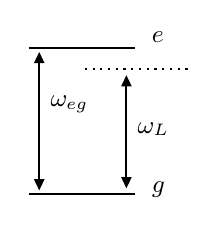
\begin{tikzpicture}[x=0.75pt,y=0.75pt,yscale=-1,xscale=1]
%uncomment if require: \path (0,121); %set diagram left start at 0, and has height of 121

%Straight Lines [id:da16867782903128048] 
\draw  [dash pattern={on 0.8pt off 2.0pt}]  (34,26) -- (84.97,26) ;
%Straight Lines [id:da39705900807308525] 
\draw    (7,86) -- (57.97,86) ;
%Straight Lines [id:da09910835469997958] 
\draw    (12.07,20.73) -- (12.07,81.36) ;
\draw [shift={(12.07,84.36)}, rotate = 270] [fill={rgb, 255:red, 0; green, 0; blue, 0 }  ][line width=0.08]  [draw opacity=0] (5.36,-2.57) -- (0,0) -- (5.36,2.57) -- cycle    ;
\draw [shift={(12.07,17.73)}, rotate = 90] [fill={rgb, 255:red, 0; green, 0; blue, 0 }  ][line width=0.08]  [draw opacity=0] (5.36,-2.57) -- (0,0) -- (5.36,2.57) -- cycle    ;
%Straight Lines [id:da027548097951511363] 
\draw    (7,16) -- (57.97,16) ;
%Straight Lines [id:da21514573737838005] 
\draw    (54.07,31.93) -- (54.07,80.36) ;
\draw [shift={(54.07,83.36)}, rotate = 270] [fill={rgb, 255:red, 0; green, 0; blue, 0 }  ][line width=0.08]  [draw opacity=0] (5.36,-2.57) -- (0,0) -- (5.36,2.57) -- cycle    ;
\draw [shift={(54.07,28.93)}, rotate = 90] [fill={rgb, 255:red, 0; green, 0; blue, 0 }  ][line width=0.08]  [draw opacity=0] (5.36,-2.57) -- (0,0) -- (5.36,2.57) -- cycle    ;

% Text Node
\draw (64.87,6.5) node [anchor=north west][inner sep=0.75pt]  [font=\small]  {$\ket{e}$};
% Text Node
\draw (64.87,78.55) node [anchor=north west][inner sep=0.75pt]  [font=\small]  {$\ket{g}$};
% Text Node
\draw (16,37.39) node [anchor=north west][inner sep=0.75pt]  [font=\small]  {$\omega _{eg}$};
% Text Node
\draw (58,50.19) node [anchor=north west][inner sep=0.75pt]  [font=\small]  {$\omega _{L}$};


\end{tikzpicture}

\end{center}

The AC Stark shift (or Autler–Townes effect) allows to create an optical lattice. Consider an atom with two energy levels and two counter-propagating laser beams in 1D (linear polarization) forming a standing wave:
%suppose also that laser's $\langle\hat{E}\rangle\sim\vec{\varepsilon}$ and 
\begin{equation*}
\begin{cases}
    \vec{\varepsilon}_1 = \varepsilon_0\cos(kx-\omega t)\vec{x}\\
    \vec{\varepsilon}_2 = \varepsilon_0\cos(-kx-\omega t)\vec{x}
\end{cases}
\end{equation*}
\begin{equation*}
\vec{\varepsilon}
= \vec{\varepsilon}_1 + \vec{\varepsilon}_2
= \vec{x} \underbrace{2\varepsilon_0\cos kx}_{\varepsilon_0(x)} \cos(\omega t) 
\end{equation*}

Let $\delta=\omega_L-\omega_{eg}$. In the condition $E_{kin} \ll \hbar\omega$, we are in the classical regime, therefore
\begin{equation*}
    H = \hbar\delta\ket{e}\bra{e}
    + \frac{\hbar\Omega(x)}{2}\hat{\sigma_x}
    + \left(
        \frac{\hbar\Omega(x)}{2}e^{2i\omega t}
        \sigma_+ 
        + h.c.
    \right)
\end{equation*}
%
and the Rabi frequency is space dependent:
$$\Omega(x) = 
\frac{\vec{d}_{eg}\cdot\vec{x}}{\hbar} 
2\varepsilon_0\cos kx $$

What's the energy of the ground (dressed) state? In the condition $\delta \gg \hbar\Omega(x)$ (large detuning) we have:
\begin{equation*}
\begin{vmatrix}
    - E & \frac{\hbar\Omega}{2}\\
    \frac{\hbar\Omega}{2} & \hbar\delta - E
\end{vmatrix}
= E^2 -\hbar\delta E - \frac{\hbar^2\Omega^2}{4} 
\stackrel{!}{=} 0
\end{equation*}
\begin{align*}
\Rightarrow \qquad 2E_g & = \hbar\delta
    - \sqrt{(\hbar\delta)^2+(\hbar\Omega)^2}
 = \hbar\delta - \hbar\delta \sqrt{1+\left(\frac{\Omega}{\delta}\right)^2} =\\
 &\stackrel{\text{expand}}{\simeq}\cancel{\hbar\delta} - \hbar\delta
    \left( \cancel{1} + \frac{\Omega^2}{2\delta^2}
    \right) =
    - \frac{\hbar\Omega^2}{2\delta}
\end{align*}

The off-resonance effect leads to the shift of ground state energy
\begin{align*}
\Delta E_g = 
- \frac{\hbar}{2\delta}
    \left( \frac{\vec{d}\cdot\hat{x} \; 4\varepsilon_0}{\hbar} \right)^2
    \cos^2{kx} = V_0 \cos^2{kx}
\end{align*}
which is like a shift of the position of the center of mass:
\begin{equation*}
\Longrightarrow \qquad H_{lattice} =  \frac{p^2}{2m} -
    \frac{V_0}{2}\cos{2kx} \;\;
    (+\;\text{const}) 
\end{equation*}

\noindent Note: Later we can check if $\omega_L \gg E_{kin}/\hbar$ is satisfied.

\noindent The atom is now in a periodic potential such that $$V(x) \sim V_0 \cos{2kx}$$ and $V_0 \sim \varepsilon_0^2/\delta$. We observe that the strength (height of barrier) is tuned by the laser power, as $I\sim|\varepsilon_0|^2$, while the sign of $\delta \lessgtr 0$ tunes the minima/maxima of the potential. Depending on the sign of $V_0$ we label the detuning as red or blue:
%
\begin{equation*}
\begin{cases}
\delta > 0 \qquad& \text{blue detuning}\\
\delta < 0 \qquad& \text{red detuning}
\end{cases}
\end{equation*}

\begin{center} \scalebox{1.5}{
    \tikzset{every picture/.style={line width=0.75pt}} %set default line width to 0.75pt        

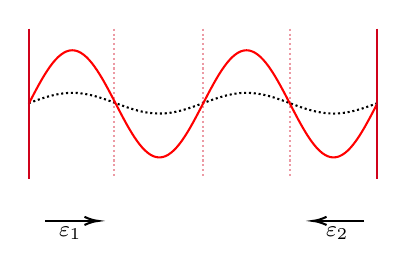
\begin{tikzpicture}[x=0.75pt,y=0.75pt,yscale=-1,xscale=1]
%uncomment if require: \path (0,120); %set diagram left start at 0, and has height of 120

%Shape: Wave [id:dp5839432983006299] 
\draw[densely dotted]   (20,41.89) .. controls (26.84,39.33) and (33.39,36.89) .. (40.98,36.89) .. controls (48.58,36.89) and (55.12,39.33) .. (61.97,41.89) .. controls (68.81,44.45) and (75.36,46.88) .. (82.95,46.88) .. controls (90.54,46.88) and (97.09,44.45) .. (103.93,41.89) .. controls (110.78,39.33) and (117.32,36.89) .. (124.92,36.89) .. controls (132.51,36.89) and (139.06,39.33) .. (145.9,41.89) .. controls (152.74,44.45) and (159.29,46.88) .. (166.88,46.88) .. controls (174.48,46.88) and (181.02,44.45) .. (187.87,41.89) ;
%Shape: Wave [id:dp906500512602781] 
\draw  [color={rgb, 255:red, 255; green, 0; blue, 0 }  ,draw opacity=1 ] (20,42.2) .. controls (26.84,28.97) and (33.39,16.38) .. (40.98,16.38) .. controls (48.58,16.38) and (55.12,28.97) .. (61.97,42.2) .. controls (68.81,55.43) and (75.36,68.02) .. (82.95,68.02) .. controls (90.54,68.02) and (97.09,55.43) .. (103.93,42.2) .. controls (110.78,28.97) and (117.32,16.38) .. (124.92,16.38) .. controls (132.51,16.38) and (139.06,28.97) .. (145.9,42.2) .. controls (152.74,55.43) and (159.29,68.02) .. (166.88,68.02) .. controls (174.48,68.02) and (181.02,55.43) .. (187.87,42.2) ;
%Straight Lines [id:da030394898450694208] 
\draw [color={rgb, 255:red, 208; green, 2; blue, 27 }  ,draw opacity=1 ]   (20,6) -- (20,78.23) ;
%Straight Lines [id:da5694280690134815] 
\draw [color={rgb, 255:red, 208; green, 2; blue, 27 }  ,draw opacity=1 ]   (187.87,6) -- (187.87,78.23) ;



%Shape: Boxed Line [id:dp8228580456036049] 
\draw [color={rgb, 255:red, 208; green, 2; blue, 27 }  ,draw opacity=.4, densely dotted ][line width=0.75]    (61.13,6) -- (61.13,78.23) ;
%Straight Lines [id:da01203909157531513] 
\draw [color={rgb, 255:red, 208; green, 2; blue, 27 }  ,draw opacity=.4, densely dotted ][line width=0.75]    (103.93,6) -- (103.93,78.23) ;
%Straight Lines [id:da23469841106616895] 
\draw [color={rgb, 255:red, 208; green, 2; blue, 27 }  ,draw opacity=.4, densely dotted ][line width=0.75]    (145.9,6) -- (145.9,78.23) ;


%Straight Lines [id:da8617246015251586] 
\draw    (28,98.6) -- (51.43,98.6) ;
\draw [shift={(53.43,98.6)}, rotate = 180] [color={rgb, 255:red, 0; green, 0; blue, 0 }  ][line width=0.75]    (6.56,-1.97) .. controls (4.17,-0.84) and (1.99,-0.18) .. (0,0) .. controls (1.99,0.18) and (4.17,0.84) .. (6.56,1.97)   ;
%Straight Lines [id:da20317114410831583] 
\draw    (181.55,98.6) -- (158.93,98.6) ;
\draw [shift={(156.93,98.6)}, rotate = 360] [color={rgb, 255:red, 0; green, 0; blue, 0 }  ][line width=0.75]    (6.56,-1.97) .. controls (4.17,-0.84) and (1.99,-0.18) .. (0,0) .. controls (1.99,0.18) and (4.17,0.84) .. (6.56,1.97)   ;

% Text Node
\draw (33.1,100) node [anchor=north west][inner sep=0.75pt]  [font=\footnotesize]  {$\varepsilon _{1}$};
% Text Node
\draw (161.8,100) node [anchor=north west][inner sep=0.75pt]  [font=\footnotesize]  {$\varepsilon _{2}$};


\end{tikzpicture}

} \end{center}

\textbf{What about energy scales?} Assume the atom is initially at rest, then it absorbs a photon from laser which transfers its momentum to the atom; the atom recoils with energy $E_R = \frac{(\hbar k)^2}{2m}$ (natural units). The different situations which can occur are:
\begin{enumerate}
    \item $E_R \gg V_0$ atoms are essentially free, they don't feel the potential
    \item $E_R \ll V_0$ atoms are trapped, confined in the potential minima
    \item $E_R \sim V_0$ atoms can tunnel from one minumum to the other
\end{enumerate}

\textbf{Observe}: The optical lattice behaves as a crystal made of light for the atoms. This is the reason we study them: they are like crystals, but can be tuned!




\vspace{1cm}










% LECTURE 24 (13 jan)

\subsection{Optical lattice in harmonic approximation}

\begin{center}
    

\tikzset{every picture/.style={line width=0.75pt}} %set default line width to 0.75pt        

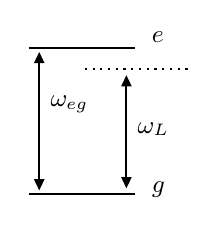
\begin{tikzpicture}[x=0.75pt,y=0.75pt,yscale=-1,xscale=1]
%uncomment if require: \path (0,121); %set diagram left start at 0, and has height of 121

%Straight Lines [id:da16867782903128048] 
\draw  [dash pattern={on 0.8pt off 2.0pt}]  (34,26) -- (84.97,26) ;
%Straight Lines [id:da39705900807308525] 
\draw    (7,86) -- (57.97,86) ;
%Straight Lines [id:da09910835469997958] 
\draw    (12.07,20.73) -- (12.07,81.36) ;
\draw [shift={(12.07,84.36)}, rotate = 270] [fill={rgb, 255:red, 0; green, 0; blue, 0 }  ][line width=0.08]  [draw opacity=0] (5.36,-2.57) -- (0,0) -- (5.36,2.57) -- cycle    ;
\draw [shift={(12.07,17.73)}, rotate = 90] [fill={rgb, 255:red, 0; green, 0; blue, 0 }  ][line width=0.08]  [draw opacity=0] (5.36,-2.57) -- (0,0) -- (5.36,2.57) -- cycle    ;
%Straight Lines [id:da027548097951511363] 
\draw    (7,16) -- (57.97,16) ;
%Straight Lines [id:da21514573737838005] 
\draw    (54.07,31.93) -- (54.07,80.36) ;
\draw [shift={(54.07,83.36)}, rotate = 270] [fill={rgb, 255:red, 0; green, 0; blue, 0 }  ][line width=0.08]  [draw opacity=0] (5.36,-2.57) -- (0,0) -- (5.36,2.57) -- cycle    ;
\draw [shift={(54.07,28.93)}, rotate = 90] [fill={rgb, 255:red, 0; green, 0; blue, 0 }  ][line width=0.08]  [draw opacity=0] (5.36,-2.57) -- (0,0) -- (5.36,2.57) -- cycle    ;

% Text Node
\draw (64.87,6.5) node [anchor=north west][inner sep=0.75pt]  [font=\small]  {$\ket{e}$};
% Text Node
\draw (64.87,78.55) node [anchor=north west][inner sep=0.75pt]  [font=\small]  {$\ket{g}$};
% Text Node
\draw (16,37.39) node [anchor=north west][inner sep=0.75pt]  [font=\small]  {$\omega _{eg}$};
% Text Node
\draw (58,50.19) node [anchor=north west][inner sep=0.75pt]  [font=\small]  {$\omega _{L}$};


\end{tikzpicture}

\end{center}

Consider a two-level atom ($\ket{g}, \ket{e}$) and two lasers, one with wave vector $k_L$ and the other with $-k_L$, counter-propagating and forming a standing wave.
Let the laser frequency be slightly detuned with respect to the transition.

\noindent We will work in the regime $\omega_L \gg \delta \gg \Omega$, so the laser frequency is much larger than the Rabi frequency and the detuning itself.
Consider also, $\omega_L$ much larger than the kinetic energy of the atom $E_K$.

In the section of AC-Stark effect we have concluded that the Hamiltonian for the center of mass of the atom, which is the 1D optical lattice Hamiltonian, is written like
\begin{equation*}
H_{lattice} =  \frac{p^2}{2m} +
    \frac{V_0}{2}\cos{2k_Lx} \;\;
    (+\;\; \text{const}) 
\end{equation*}
where we have actually changed the sign in front of $V_0$. Recall that the sign depends on the detuning, whether it is red or blue.

We have already discussed three regimes, depending on the ratio of the recoil energy $E_R$ and the potential strenght $V_0$. In this section we will address the case $E_R \ll V_0$.


\begin{tcolorbox}[breakable, enhanced]
\textbf{Example}\\

Let us take, for instance, the Rubidium 87 and a laser with $\lambda = 2\pi/k_L = 852 nm$. This frequency will be slightly detuned wrt a transition from ground state $S$ to an excited $P$ (which will be some hyper-fine structure level). 

\begin{itemize}
    \item The recoil energy would be $E_R \sim 3.2 kHz$. Indeed, it is $\ll$ optical frequencies, which range around $\sim THz$.
    \item If we consider the atom at a temperature of few hundred $nK$, we would get a kinetic energy which is smaller than $E_R$.\\
\end{itemize}

All the conditions we have defined above are satisfied!\\

\noindent \textbf{Question}: \textit{Do we care whether the excited level is long-lived or not?} No, we don't care, because $\delta \gg \Omega$, so we are not populating this level. Nevertheless, the lifetime actually determines the width of the energy level; therefore the laser detuning must be sufficiently larger than the width of the atomic level.
\end{tcolorbox}


As already discussed, $E_R \ll V_0$ means that the atom will feel a large potential barrier with little chance to escape from it, then it is basically localised at the minima of potential. \textbf{Our goal is to compare the harmonic oscillator size $\xi$ with the lattice spacing}\footnote{
Lattice spacing comes from the periodicity of $\cos(2k_Lx)$. We also observe that it is in the order of $100 nm$, because it is an optical transition. Solids have fractions of nanometer spacing, usually!
}
$$a=\pi/k_L \;\;$$



In order to do so, let us expand the potential $V(x)$ in the harmonic approximation around a minima $x_n$. This approximation will allow us to describe physics inside a single well, but in general it will not be satisfying when considering all the wells.

\begin{center}
\scalebox{1.4}{
    

\tikzset{every picture/.style={line width=0.75pt}} %set default line width to 0.75pt        

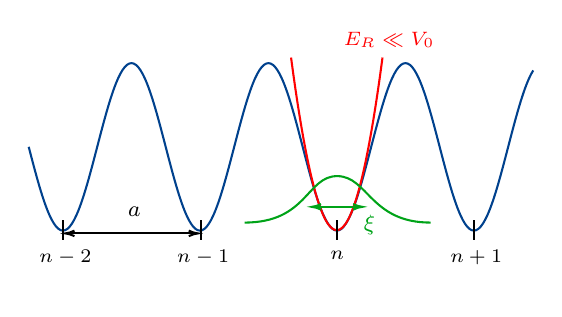
\begin{tikzpicture}[x=0.75pt,y=0.75pt,yscale=-1,xscale=1]
%uncomment if require: \path (0,135); %set diagram left start at 0, and has height of 135

%Shape: Wave [id:dp5948468038024646] 
\draw  [color={rgb, 255:red, 0; green, 65; blue, 141 }  ,draw opacity=1 ] (12,69.53) .. controls (17.38,90.2) and (22.53,109.88) .. (28.5,109.88) .. controls (34.47,109.88) and (39.62,90.2) .. (45,69.53) .. controls (50.38,48.86) and (55.53,29.18) .. (61.5,29.18) .. controls (67.47,29.18) and (72.62,48.86) .. (78,69.53) .. controls (83.38,90.2) and (88.53,109.88) .. (94.5,109.88) .. controls (100.47,109.88) and (105.62,90.2) .. (111,69.53) .. controls (116.38,48.86) and (121.53,29.18) .. (127.5,29.18) .. controls (133.47,29.18) and (138.62,48.86) .. (144,69.53) .. controls (149.38,90.2) and (154.53,109.88) .. (160.5,109.88) .. controls (166.47,109.88) and (171.62,90.2) .. (177,69.53) .. controls (182.38,48.86) and (187.53,29.18) .. (193.5,29.18) .. controls (199.47,29.18) and (204.62,48.86) .. (210,69.53) .. controls (215.38,90.2) and (220.53,109.88) .. (226.5,109.88) .. controls (232.47,109.88) and (237.62,90.2) .. (243,69.53) .. controls (247.01,54.12) and (250.9,39.25) .. (255.09,32.69) ;
%Shape: Parabola [id:dp32380929671166225] 
\draw  [color={rgb, 255:red, 255; green, 0; blue, 0 }  ,draw opacity=1 ] (138.4,26.5) .. controls (153.08,137.41) and (167.77,137.41) .. (182.45,26.5) ;
%Straight Lines [id:da20114798739595108] 
\draw    (31.67,111.22) -- (91.49,111.22) ;
\draw [shift={(93.49,111.22)}, rotate = 180] [color={rgb, 255:red, 0; green, 0; blue, 0 }  ][line width=0.75]    (4.37,-1.32) .. controls (2.78,-0.56) and (1.32,-0.12) .. (0,0) .. controls (1.32,0.12) and (2.78,0.56) .. (4.37,1.32)   ;
\draw [shift={(29.67,111.22)}, rotate = 0] [color={rgb, 255:red, 0; green, 0; blue, 0 }  ][line width=0.75]    (4.37,-1.32) .. controls (2.78,-0.56) and (1.32,-0.12) .. (0,0) .. controls (1.32,0.12) and (2.78,0.56) .. (4.37,1.32)   ;
%Straight Lines [id:da9743703357911851] 
\draw    (28.4,105) -- (28.4,114.51) ;

%Straight Lines [id:da7045788488223218] 
\draw    (94.8,105) -- (94.8,114.51) ;

%Straight Lines [id:da9576353190403918] 
\draw    (226.4,105) -- (226.4,114.51) ;

%Straight Lines [id:da19564966071273038] 
\draw    (160.4,105) -- (160.4,114.51) ;
%Curve Lines [id:da7613317075373456] 
\draw [color={rgb, 255:red, 0; green, 163; blue, 24 }  ,draw opacity=1 ]   (116,106) .. controls (146.29,106.02) and (145.91,83.51) .. (160.69,83.62) .. controls (175.46,83.73) and (176.69,106.02) .. (205.6,106) ;
%Straight Lines [id:da49305309064742076] 
\draw [color={rgb, 255:red, 0; green, 163; blue, 24 }  ,draw opacity=1 ]   (150.47,98.42) -- (170.69,98.42) ;
\draw [shift={(172.69,98.42)}, rotate = 180] [color={rgb, 255:red, 0; green, 163; blue, 24 }  ,draw opacity=1 ][line width=0.75]    (4.37,-1.32) .. controls (2.78,-0.56) and (1.32,-0.12) .. (0,0) .. controls (1.32,0.12) and (2.78,0.56) .. (4.37,1.32)   ;
\draw [shift={(148.47,98.42)}, rotate = 0] [color={rgb, 255:red, 0; green, 163; blue, 24 }  ,draw opacity=1 ][line width=0.75]    (4.37,-1.32) .. controls (2.78,-0.56) and (1.32,-0.12) .. (0,0) .. controls (1.32,0.12) and (2.78,0.56) .. (4.37,1.32)   ;

% Text Node
\draw (58.4,97) node [anchor=north west][inner sep=0.75pt]  [font=\footnotesize]  {$a$};
% Text Node
\draw (15.6,117.89) node [anchor=north west][inner sep=0.75pt]  [font=\scriptsize]  {$n-2$};
% Text Node
\draw (82,117.89) node [anchor=north west][inner sep=0.75pt]  [font=\scriptsize]  {$n-1$};
% Text Node
\draw (213.6,117.89) node [anchor=north west][inner sep=0.75pt]  [font=\scriptsize]  {$n+1$};
% Text Node
\draw (155.8,118.09) node [anchor=north west][inner sep=0.75pt]  [font=\scriptsize]  {$n$};
% Text Node
\draw (162.4,12.6) node [anchor=north west][inner sep=0.75pt]  [font=\scriptsize,color={rgb, 255:red, 255; green, 0; blue, 0 }  ,opacity=1 ]  {$E_{R} \ll V_{0}$};
% Text Node
\draw (172,101) node [anchor=north west][inner sep=0.75pt]  [font=\footnotesize,color={rgb, 255:red, 0; green, 163; blue, 24 }  ,opacity=1 ]  {$\xi $};


\end{tikzpicture}

}
\end{center}


The expansion of the potential around the $n$th minima $x_n$ (but let's focus around $n=0$), we get
\begin{equation*}
    V(x) = \sum_n V(x-x_n) \simeq
    - \underbrace{
        \frac{V_0}{2}\left(
        1 - \frac{(2kx)^2}{2} + \dots
        \right)
    }_{n=0}
    + \underbrace{\dots}_{n\neq 0}
\end{equation*}
so we can rewrite the potential of the lattice Hamiltonian (around site $x_n$) as
\begin{equation*}
    H \simeq \frac{p^2}{2m} + V_0k^2x^2
\end{equation*}

\noindent Comparing the potential with its usual representation as function of $\omega_{osc}$, $$\frac{1}{2}m\omega_{osc}^2 = V_0k^2$$
therefore
$$\omega_{osc} = \sqrt{\frac{2V_0}{m}}\;k = 
\sqrt{4V_0\frac{k^2}{2m}} = \frac{2}{\hbar}\sqrt{V_0E_R}$$

\noindent Therefore, the size (or length-scale) $\xi$ of the harmonic oscillator is
$$\xi = \frac{\hbar}{\sqrt{m\omega_{osc}}}$$

\begin{equation*}
    \Longrightarrow \;\;
    \frac{\xi^2}{a^2} = \frac{\hbar^2}{m\omega_{osc}}\frac{k^2}{\pi^2}=
    \frac{1}{\pi^2}\sqrt{\frac{E_R}{V_0}}
\end{equation*}
    
When $V_0$ is very large then the harmonic oscillator spacing is much smaller than the lattice spacing, $\xi \ll a$. In this regime, the harmonic oscillator is a good approximation.



\begin{tcolorbox}[breakable, enhanced]
\textbf{Example}\\

For Rubidium,
$V_0 \simeq 20 E_R$,
$\;\omega_{osc} \simeq 28 \text{kHz}\;$
and $\;\xi/a = 0.15$.
\end{tcolorbox}





\section{Energy bands}


However, we would like to move beyond the harmonic approximation.
When $V_0$ is of the order of the $E_R$, indeed, the harmonic oscillator picture does not work anymore.
We will have to resort to the machinery of solid state physics, so the concept of energy bands. We will review it today for the case of the optical lattice. \\
\textbf{What's the spectrum in this new regime?} It is not the harmonic oscillator spectrum anymore, because now each well is not fully independent. Anyway, we still stay in the few hundred nano-Kelvin regime, which is enough to stay on the lowest harmonic oscillator level.





The most general problem we want to solve is
$$H=\frac{p^2}{2m} + V(x)$$
where $V : V(x) = V(x+a)$ is a periodic potential.

The \textit{Bloch theorem} assures that the solutions of this problem are of the form:
$$\psi_q(x) = e^{iqx}u_q(x)$$
where $u_q(x+a) = u_q(x)$
for $q\in [-\frac{\pi}{a},\frac{\pi}{a}[$ (which is called \textit{first Brillouin zone}).


\noindent We insert the prototype of the solution in the Schrödinger equation:
\begin{equation}
\label{eq:proto-schr-energy-bands}
\left(
    -\frac{\hbar^2}{2m}\partial^2_x -\frac{V_0}{2}\cos(2kx)
\right)
e^{iqx} u_q(x)
= E e^{iqx} u_q(x)
\end{equation}

\noindent Since $V$ is periodic, we can use the Fourier decomposition\footnote{
This method is suitable for optical lattices, but in general is not largely used in solid state physics. There are still other methods to address the most general cases, but now we can take into account that the potential is periodic. In this case it is very convenient to do a Fourier decomposition, as $\cos kx$ is easy to expand, and will lead to simple results, too.}
\begin{equation*}
    u_q(x)=\sum_{n=-\infty}^{+\infty}
    c_n e^{i\frac{2\pi}{a}nx}
    \;\;, \qquad n \in \mathbb{Z}
\end{equation*}

\noindent The LHS of Eq. is \ref{eq:proto-schr-energy-bands} is
\begin{align*}
&\sum_{n=-\infty}^{+\infty}
\left(
    -\frac{\hbar^2}{2m}\partial^2_x -\frac{V_0}{4}
    \left(e^{i2kx} + e^{-i2kx}\right)
\right)
\exp{i\left(\frac{2\pi}{a}n+q\right)x} c_n =\\
% applying operators
& =\sum_{n} \left(
    \frac{\hbar^2}{2m}
    \left(\frac{2\pi}{a}n+q\right)^2
    -\frac{V_0}{4}
    \left(e^{i2kx} + e^{-i2kx}\right)
\right)
e^{i\left(\frac{2\pi}{a}n+q\right)x} c_n 
\equalexpl{$k=\pi/a$} \\
% breaking in two pieces
& = \sum_{n} \left(
    \frac{\hbar^2}{2m}\left(\frac{2\pi}{a}n+q\right)^2
\right) e^{i\left(\frac{2\pi}{a}n+q\right)x} c_n
-
\sum_{n} \frac{V_0}{4} \left(
    e^{i\frac{2\pi}{a}(n+1)x}
    + e^{-i\frac{2\pi}{a}(n-1)x}
\right) e^{iqx} c_n
\end{align*}


\noindent Considering also the RHS, simplifying $e^{iqx}$ and suitably shifting the sums at LHS ($n+1\rightarrow n$, $n-1 \rightarrow n$), we get
\begin{align*}
\sum_{n} \left(
    \frac{\hbar^2}{2m}\left(\frac{2\pi}{a}n+q\right)^2
\right) e^{i\frac{2\pi}{a}nx} c_n
-
\frac{V_0}{4} \sum_{n}  \left(
    e^{i\frac{2\pi}{a}nx}
    \left( c_{n-1} + c_{n+1} \right)
\right) =
\sum_{n} E e^{i\frac{2\pi}{a}nx} c_n
\end{align*}
which we can rewrite as
\begin{equation*}
\sum_{n}
\left( \; \dots \; \right)
 _{n, n+1, n-1}
 e^{i\frac{2\pi}{a}nx} = 0 \:\:.
\end{equation*}

\noindent This is true $ \Leftrightarrow \left( \; \dots \; \right) = 0 \; \forall n$ - due to the orthogonality of Fourier basis - i.e.
\begin{equation*}
\frac{\hbar^2}{2m}
\left(\frac{2\pi}{a}n+q\right)^2 c_n
- \frac{V_0}{4} \left( c_{n+1} + c_{n-1} \right)
= E c_n
\end{equation*}

\noindent Applying the change of variable $\tilde{q} = q/(\pi/a)$, with $q\in[-\pi/a, \pi/a[ \;\Rightarrow\; \tilde{q} \in [-1,1[$,

\begin{equation}
\label{eq:final-bands}
\Rightarrow \; 
\underbrace{\frac{\hbar^2 (\pi/a)^2}{2m}}
_{= E_R}
\left(2n+\tilde{q}\right)^2 c_n
- \frac{V_0}{4} \left( c_{n+1} + c_{n-1} \right)
= E c_n
\end{equation}

\noindent A few observations:
\begin{itemize}
\item The solution of this eigenvalue problem will be all the possible energies that the particle in a periodic potential can take. However, you cannot solve it analytically. One can approach the problem perturbatively (Ashcroft-Mermin), for instance, when $V_0$ is small. But we are really interested in the regime $V_0 \simeq E_R$, so we have no other choice than solving it numerically.
\item We notice that there is a recoil energy, which appears to be the only relevant energy for this computation. Dividing everything by $E_R$, we would solve the problem with energy in units of $E_R$.
\item If written in matrix form, the LHS appears to be a tridiagonal matrix,
\begin{equation*}
    \begin{pmatrix}
    \ddots & \ddots\\
    \ddots & \tilde{q}-2n & -V_0/4    & 0\\
           & -V_0/4       & \tilde{q} & -V_0/4\\
           & 0            & -V_0/4    & \tilde{q}+2n & \ddots\\
           &              &           & \ddots       & \ddots
    \end{pmatrix}
\end{equation*}
This is due to the Fourier expansion of the cosine in the potential, which selects just few Fourier harmonics, leading to this sparse form of the eigenvalue problem.

\end{itemize}

\noindent Even though the solution cannot be obtained analytically, we can still try to visualise what happens. In absence of potential ($V_0 = 0$), we get the free-particle spectrum\footnote{
    Recall that $q$ is a full momentum. We have considered natural units, $\hbar = 1$.}
$$E(q) = \frac{q^2}{2m}$$
which is a simple parabola. Comparing with a numerical solution (Figure \ref{fig:numerical-bands}), we would see that for $V_0 \neq 0$ appear some gaps in correspondence of the crystal momenta $\pi/a$, $2\pi/a$, $\dots$

\begin{figure}[H]
  \centering
  \subfloat[Unfolded view]{\includegraphics[width=0.66\textwidth]{img/unfolded.pdf}\label{fig:numerical-bands-unfolded}}
  \hfill
  \subfloat[Folded view]{\includegraphics[width=0.33\textwidth]{img/folded.pdf}\label{fig:numerical-bands-folded}}
  \caption{\label{fig:numerical-bands} 
Numerical solution of Eq. \ref{eq:final-bands}, for different values of $V_0$. 
The curve for $V_0 = 0$ (black line) is the free-particle spectrum (a parabola in the momenta $q$). 
For $V_0\neq 0$ appear discontinuities in correspondence of $q=\pi/a, 2\pi/a, \dots$
The discontinuities are called \textbf{gaps}. We notice that the gaps get smaller as we increase the momenta: this is due to the increasing free particle energy, which becomes dominant, so the particle behaves like the lattice is not there.\\ \textit{That's when you can slide objects on top of tables and they don't get stuck!}\\
The subplot \textit{b} shows the same numerical result but folded in the first Brillouin zone. Indeed, due to the periodicity conditions to the solution to the Schrodinger equation, $\psi(q)$ would have the same value when shifting the momentum by $2\pi/a$. So a more convenient representation would not be the one in which $q$ ranges all real numbers, but the one which maps all momentums to the first Brillouin zone ($-\pi/a, \pi/a$) with shifts of $2\pi/a$. This is called \textbf{folding}. 
}
\end{figure}


\noindent \textbf{Take-away message}: When $V_0 \neq 0$ \textbf{the energies are compacted into bands} and there appear gaps.
A gap means that for those momenta there is not allowed state for the particle/atom/system.







\subsection{Tight-binding limit}

For large enough $V_0$ (larger than $E_R$). In this regime, we expect particles to be sufficiently localised in each well, but can also tunnel to the next well, jumping to the next minimum of the potential.

Instead of using the Block functions (the Bloch theorem solutions $\psi_{\alpha q}(x)$), we will use the harmonic oscillator solutions $\phi_\nu(x - x_n)$ to build a basis for the potential.

\begin{tcolorbox}[breakable, enhanced]
\begin{minipage}{0.45\textwidth}
\begin{center}
    $\psi_{\alpha q}(x)$

    $\alpha$ is the index of the band
\end{center}

    Ranging on all $\alpha$s and on all $q$s one has a complete set of wave-functions.
\end{minipage}\hfill
\begin{minipage}{0.45\textwidth}
\begin{center}
    $\phi_\nu(x - x_n)$

    $\nu$ harmonic energy level in the minimum $x_n$
\end{center}

    SPOILER: This does \textbf{not} form a basis!
\end{minipage}
\end{tcolorbox}



However, the harmonic oscillator wave-functions are not a basis. We can show that
$$\langle \phi_\nu (x-x_n) | \phi_\mu(x-x_n) \rangle = \delta_{\mu\nu}$$
so they behave like a basis for a single minima potential $x_n$.

But what if we fix $\nu$ and $\mu$, $\nu = \mu = 1$ for instance? The, the family of harmonic oscillator wave-functions in different wells ($x_n$ and $x_{n'}$) are not a basis. Indeed
$$\langle \phi_1 (x-x_n) | \phi_1(x-x_{n'}) \rangle
= \int dx \phi^*(x-x_n)\phi(x-x_{n'}) > 0 \qquad \text{for}\;\; n \neq n'$$
The last inequality comes from 
$\phi_1 (x-x_n) \propto e^{-x^2/\varepsilon^2} > 0$.
%
We conclude that \textbf{the family of harmonic oscillator wave-functions can be a good approximation, but they are not a perfect solution of the problem}\footnote{
    This is not a surprise... our potential is a cosine, the harmonic functions are just a mere approximation of it.}.
%
Instead, we want to find a basis, i.e. a set of functions solving the full problem or spanning the full space of wave-functions.\\


We already know the basis of Bloch functions $\psi_{\alpha q}(x)$. We now build a new basis from it performing a unitary transformation.\\

Let us define the \textbf{Wannier basis}, applying a Fourier transform on $\psi_{\alpha q}(x)$:
\begin{equation*}
w_\alpha(x-x_n) = \frac{1}{\sqrt{N_s}}
\sum_q e^{-iqx_n}\psi_{\alpha q}(x)
\end{equation*}
This is a valid transformation only for isolated bands. If the bands touch somewhere, then we have a degeneracy and it requires a particular treatment\footnote{
    There is a talk on YouTube (\href{https://www.youtube.com/watch?v=eHyqkB4ZMjw}{youtube.com/watch?v=eHyqkB4ZMjw}) by Giovanni Pizzi on this topic.
}.
%
One can prove that:
\begin{itemize}
\setlength\itemsep{1mm}
    \item $w_\alpha$ depends only on $x-x_n$
    \item $\langle w_\alpha(x-x_n) | w_\beta(x-x_{n'})\rangle = \delta_{\alpha\beta}\delta_{n n'}$, since the $u_q(x)$ are orthogonal
\end{itemize}

\noindent Our goal is to simplify the expression as much as possible, since there is the freedom
$$\psi_{\alpha q}(x) \longrightarrow \psi_{\alpha q}(x)e^{i\theta(q)}$$
because those functions
\begin{itemize}
\setlength\itemsep{1mm}
    \item are solutions to the same Schrodinger equations
    \item generate different set of Wannier $w_\alpha$
\end{itemize}


\noindent W. Kohn studied condensed matter and discovered (1959) that if $V(x)=V(-x)$ (inversion condition), then for each isolated $\alpha$ band $ \exists! w_\alpha(x-x_n)\;\; \forall n$ that is:
\begin{itemize}
\setlength\itemsep{1mm}
    \item real
    \item symmetric or anti-symmetric
    \item falling off exponentially with distance, i.e. $w_\alpha(x) \sim e^{-\hbar x^2}$ for large $x$
\end{itemize}

This result assures that there exist only one Wannier for each band which minimizes the $\psi$ at each site: there is no ambiguity in determining the Wannier basis! Furthermore, they are also exponentially localized, which allows us to do some simplification in the choice of the Wannier functions.

Instead of solving the problem using as many Wannier functions as you want (this is in principle the most general approach), under our assumptions, one can use just one or two of them. Indeed, since the Wannier functions are exponentially localized, one can associate them to a length scale. For a suitable choice, this length scale can be sufficiently small compared to the lattice periodicity.

Wannier states are orthogonal, but they are not eigenstates for the basis in which the Hamiltonian is written. The Hamiltonian elements in terms of the Wannier functions are
$$ - J_{j,j'}^{(\alpha,\beta)} \equiv \langle w_\alpha(x_j)|\hat{H}|w_\beta(x_{j'}) \rangle$$






% LECTURE 25 (19 jan)

\noindent Considering the lowest band, the related Wannier functions have $\alpha = 1$; therefore, let us define $\ket{j} = \ket{w_{\alpha=1}(x_j)}$. If and only if there is an appropriate energy separation ($T$, interactions $\ll$ gap), we can restrict the dynamics to the lowest band and write the hamiltonian as
\begin{equation}
\label{eq:tight-band-all}
    \Rightarrow \hat{H}_{TB} = -\sum_{j,\mu} J_{j,j+\mu}^{(1,1)} \left[ \ket{j}\bra{j+\mu} + h.c. \right]
\end{equation}
%
We can further simplify the expression: since $w(x_j)$ are exponentially localized, the overlap between functions is almost null if the functions are sufficiently separated $\Leftrightarrow \mu$ is sufficiently large.

\begin{center}
    \scalebox{1.4}{ 
\tikzset{every picture/.style={line width=0.75pt}} %set default line width to 0.75pt        

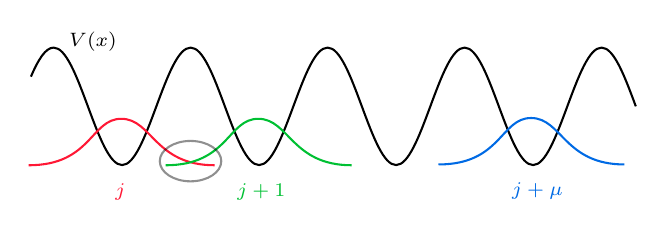
\begin{tikzpicture}[x=0.75pt,y=0.75pt,yscale=-1,xscale=1]
%uncomment if require: \path (0,100); %set diagram left start at 0, and has height of 100

%Shape: Wave [id:dp1124656768591269] 
\draw  [color={rgb, 255:red, 0; green, 0; blue, 0 }  ,draw opacity=1 ] (300.5,44.62) .. controls (295.11,30.13) and (289.97,16.32) .. (284,16.32) .. controls (278.02,16.32) and (272.88,30.13) .. (267.5,44.62) .. controls (262.11,59.12) and (256.97,72.92) .. (251,72.92) .. controls (245.02,72.92) and (239.88,59.12) .. (234.5,44.62) .. controls (229.11,30.13) and (223.97,16.32) .. (218,16.32) .. controls (212.02,16.32) and (206.88,30.13) .. (201.5,44.62) .. controls (196.11,59.12) and (190.97,72.92) .. (185,72.92) .. controls (179.02,72.92) and (173.88,59.12) .. (168.5,44.62) .. controls (163.11,30.13) and (157.97,16.32) .. (152,16.32) .. controls (146.02,16.32) and (140.88,30.13) .. (135.5,44.62) .. controls (130.11,59.12) and (124.97,72.92) .. (119,72.92) .. controls (113.02,72.92) and (107.88,59.12) .. (102.5,44.62) .. controls (97.11,30.13) and (91.97,16.32) .. (86,16.32) .. controls (80.02,16.32) and (74.88,30.13) .. (69.5,44.62) .. controls (64.11,59.12) and (58.97,72.92) .. (53,72.92) .. controls (47.02,72.92) and (41.88,59.12) .. (36.5,44.62) .. controls (31.11,30.13) and (25.97,16.32) .. (20,16.32) .. controls (16.1,16.32) and (12.55,22.2) .. (9.07,30.31) ;
%Curve Lines [id:da06441510036165143] 
\draw [color={rgb, 255:red, 255; green, 24; blue, 53 }  ,draw opacity=1 ]   (8,73) .. controls (38.29,73.02) and (37.91,50.51) .. (52.69,50.62) .. controls (67.46,50.73) and (68.69,73.02) .. (97.6,73) ;
%Curve Lines [id:da10660086824458115] 
\draw [color={rgb, 255:red, 0; green, 192; blue, 51 }  ,draw opacity=1 ]   (74,73) .. controls (104.29,73.02) and (103.91,50.51) .. (118.69,50.62) .. controls (133.46,50.73) and (134.69,73.02) .. (163.6,73) ;
%Curve Lines [id:da5007784416198438] 
\draw [color={rgb, 255:red, 0; green, 106; blue, 228 }  ,draw opacity=1 ]   (205.43,72.62) .. controls (235.72,72.64) and (235.34,50.13) .. (250.12,50.24) .. controls (264.89,50.34) and (266.12,72.64) .. (295.03,72.62) ;
%Shape: Ellipse [id:dp01210222813331252] 
\draw  [color={rgb, 255:red, 0; green, 0; blue, 0 }  ,draw opacity=0.44 ][line width=0.75]  (71.14,71.02) .. controls (71.14,65.64) and (77.78,61.29) .. (85.96,61.29) .. controls (94.15,61.29) and (100.78,65.64) .. (100.78,71.02) .. controls (100.78,76.39) and (94.15,80.75) .. (85.96,80.75) .. controls (77.78,80.75) and (71.14,76.39) .. (71.14,71.02) -- cycle ;

% Text Node
\draw (48.09,80.52) node [anchor=north west][inner sep=0.75pt]  [font=\scriptsize,color={rgb, 255:red, 255; green, 24; blue, 53 }  ,opacity=1 ]  {$j$};
% Text Node
\draw (106.89,80.32) node [anchor=north west][inner sep=0.75pt]  [font=\scriptsize,color={rgb, 255:red, 0; green, 192; blue, 51 }  ,opacity=1 ]  {$j+1$};
% Text Node
\draw (239.31,79.93) node [anchor=north west][inner sep=0.75pt]  [font=\scriptsize,color={rgb, 255:red, 0; green, 106; blue, 228 }  ,opacity=1 ]  {$j+\mu $};
% Text Node
\draw (26,7.22) node [anchor=north west][inner sep=0.75pt]  [font=\scriptsize]  {$V( x)$};


\end{tikzpicture}
 }
\end{center}

We remark that the Wannier functions are orthogonal, but there could be matrix elements outside the diagonal.
However, the dominant matrix elements will be the ones with largest overlap. For example, we can consider that $J_{j,j'} \gg J_{j,j+3}$ and then only small values of $\mu$ are taken into account for the case of $V_0 \gg E_R$.\\

If we take the Fourier transform, quantized over $jk$ and assuming periodic bound conditions,
\begin{equation}
\label{eq:tight-basis-def}
    \ket{k} = \frac{1}{\sqrt{N_s}}\sum_j e^{-ijka}\ket{j} \qquad\qquad \text{where}\;\; ja = \frac{2\pi}{N_s}n,\;\; n\in[0,N_s-1]
\end{equation}
%
\noindent It is easy to prove that $\{\ket{k}\}$ are an orthogonal set and that it is normalized to one: projecting on another Bloch wave-vector $\bra{q}$, $\Rightarrow$
\begin{align}
    \bra{q}\ket{k} &= \frac{1}{N_s} \sum_{j,j'} e^{ikqa}\bra{j}\ket{j'}e^{-ikj'a} 
    = \frac{1}{N_s} \sum_{j,j'} \delta_{j,j'} e^{ikja}e^{-iqj'a}
    = \frac{1}{N_s} \sum_j e^{i(k-q)ja}\nonumber\\
    &= \frac{1}{N_s}
    \begin{cases}
        N_s& \text{if}\; k=q\\
        0 &\text{else}  \qquad \longleftarrow \text{all the momenta are out of phase}
    \end{cases}
    \label{eq:phase-sum}
\end{align}



The hamiltonian \ref{eq:tight-band-all} can be rewritten in the momentum space as
\begin{equation}
\label{eq:tight-band-momentum}
    \hat{H}_{TB} = -\sum_{j,\mu} J_{j,j+\mu}\left( \ket{j}\bra{j+\mu} + h.c. \right)
\end{equation}
Remember that this expression is considering only the lowest energy band. We want to study its spectrum, which means to diagonalize the hamiltonian.

First, we notice that the Wannier functions are real (in a suitable gauge), so all of the hamiltonian matrix elements are real numbers.

\noindent Second, because all lattice sites are physically equivalent, we consider the translational symmetry to consider the $J$ as functions of $\mu$ only:
\begin{equation*}
    J_{j.j+\mu} \equiv J_\mu \qquad (\in \mathcal{R}) \;.
\end{equation*}

\noindent We now can diagonalize the hamiltonian


\begin{align*}
    \Longrightarrow \hat{H}_{TB} &\overset{\ref{eq:tight-band-momentum}}{=} -\sum_{j,\mu} J_{j.j+\mu}
    \left( \ket{j}\bra{j+\mu} + h.c. \right)
        \overset{\text{\ref{eq:tight-basis-def}}}{=}\\
    &= -\sum_{j,\mu} \frac{1}{N_s}\sum_k\sum_q  J_\mu e^{+i(j)ka} e^{-i(j+\mu)qa} \ket{k}\bra{q} + h.c. = \\
    &= - \frac{1}{N_s}\sum_{\mu,k,q}
        J_\mu \underbrace{\sum_{j} e^{ija(k-q)}}_{=\delta_{k,q}\cdot N_s \;\; \text{(\ref{eq:phase-sum})}} e^{-i\mu qa} \ket{k}\bra{q} + h.c. =\\
    &= -\sum_\mu\sum_k J_\mu
        \left( e^{-ik\mu a} \ket{k}\bra{k} + e^{ik\mu a} \ket{k}\bra{k} \right) =\\
    &= -\sum_{k,\mu} J_\mu \cdot 2\cos(\mu ka) \ket{k}\bra{k} \equiv \sum_k E(k) \ket{k}\bra{k}
\end{align*}
but we care only about the spectrum (eigenvalues):
\begin{equation}
\label{eq:spectrum-tight-binding}
    E(k) = -2\sum_\mu J_\mu \cos{(\mu ka)}
\end{equation}

In the tight-binding limit, we can neglect higher values of $\mu$. For example, we set $J_\mu = 0$, say, for $\mu > 2$; then $E(k) \simeq -2J_1 \cos{(ka)} -2J_2 \cos{(2ka)}$.
%
We can be more severe and ignore $J_\mu$ for $\mu > 1$, because $J_1 \gg J_2 \gg J_3 \gg \dots$ by orders of magnitude due to the exponential localization of Wannier functions. Doing this, the spectrum is completely determined by $J_1$ itself

\begin{minipage}{0.50\textwidth}
    \begin{center}
    \scalebox{0.95}{ 

\tikzset{every picture/.style={line width=0.75pt}} %set default line width to 0.75pt        

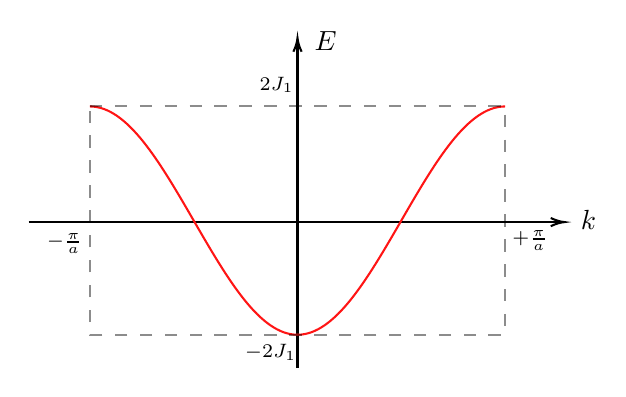
\begin{tikzpicture}[x=0.75pt,y=0.75pt,yscale=-1,xscale=1]
%uncomment if require: \path (0,175); %set diagram left start at 0, and has height of 175

%Straight Lines [id:da4301961974434454] 
\draw    (140,169.21) -- (140,12.2) ;
\draw [shift={(140,10.2)}, rotate = 90] [color={rgb, 255:red, 0; green, 0; blue, 0 }  ][line width=0.75]    (6.56,-1.97) .. controls (4.17,-0.84) and (1.99,-0.18) .. (0,0) .. controls (1.99,0.18) and (4.17,0.84) .. (6.56,1.97)   ;
%Straight Lines [id:da644600047896886] 
\draw    (10.5,98.86) -- (266.57,98.86) ;
\draw [shift={(268.57,98.86)}, rotate = 180] [color={rgb, 255:red, 0; green, 0; blue, 0 }  ][line width=0.75]    (6.56,-1.97) .. controls (4.17,-0.84) and (1.99,-0.18) .. (0,0) .. controls (1.99,0.18) and (4.17,0.84) .. (6.56,1.97)   ;
%Shape: Wave [id:dp8332830628724615] 
\draw  [color={rgb, 255:red, 255; green, 21; blue, 21 }  ,draw opacity=1 ] (40,43.14) .. controls (58.1,43.14) and (73.69,69.97) .. (90,98.14) .. controls (106.31,126.32) and (121.9,153.14) .. (140,153.14) .. controls (158.1,153.14) and (173.69,126.32) .. (190,98.14) .. controls (206.31,69.97) and (221.9,43.14) .. (240,43.14) ;
%Shape: Rectangle [id:dp8283156136322417] 
\draw  [color={rgb, 255:red, 0; green, 0; blue, 0 }  ,draw opacity=0.45 ][dash pattern={on 4.5pt off 4.5pt}] (40,43.1) -- (240,43.1) -- (240,153.1) -- (40,153.1) -- cycle ;

% Text Node
\draw (275,91.83) node [anchor=north west][inner sep=0.75pt]  [font=\normalsize]  {$k$};
% Text Node
\draw (146.79,5.69) node [anchor=north west][inner sep=0.75pt]  [font=\normalsize]  {$E$};
% Text Node
\draw (17.71,102.83) node [anchor=north west][inner sep=0.75pt]  [font=\scriptsize]  {$-\frac{\pi }{a}$};
% Text Node
\draw (242,101.4) node [anchor=north west][inner sep=0.75pt]  [font=\scriptsize]  {$+\frac{\pi }{a}$};
% Text Node
\draw (120.29,27.4) node [anchor=north west][inner sep=0.75pt]  [font=\scriptsize]  {$2J_{1}$};
% Text Node
\draw (113.14,156.26) node [anchor=north west][inner sep=0.75pt]  [font=\scriptsize]  {$-2J_{1}$};


\end{tikzpicture}
 }
    \end{center}
\end{minipage}\hfill
\begin{minipage}{0.40\textwidth}
    and the bandwidth is
    \begin{align*}
        \Delta E &= E\left(k=\frac{\pi}{a}\right) - E\left(k=0\right)\\
        &= 2J_1 - (- 2J_1) = 4J_1
    \end{align*}
\end{minipage}


\begin{tcolorbox}[breakable, enhanced]
\textbf{Recap}\\

In the tight-binding limit, the potential is sufficiently deep and the bands are sufficiently separated. Under these circumstances, the lattice is able to confine the wave-function to a single site. The lowest band of an atom in a lattice is described by the (nearest-neighbor) hamiltonian
\begin{equation*}
    \hat{H}_{TB} = -J\sum_j
    \left( \ket{j}\bra{j+1} + \ket{j+1}\bra{j}\right)
\end{equation*}

The amplitude of the hopping (or tunneling) process is basically $J\simeq J_1$. The transmission is not exactly like the problem you have seen in an introductory course on Quantum Mechanics, but it is really similar.

\begin{center}
    \scalebox{1.2}{ 

\tikzset{every picture/.style={line width=0.75pt}} %set default line width to 0.75pt        

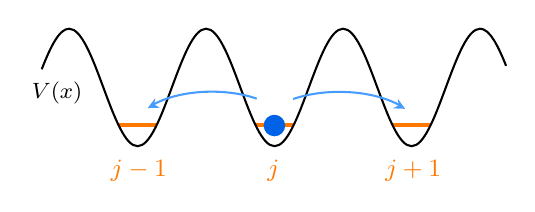
\begin{tikzpicture}[x=0.75pt,y=0.75pt,yscale=-1,xscale=1]
%uncomment if require: \path (0,100); %set diagram left start at 0, and has height of 100

%Straight Lines [id:da8895757852919295] 
\draw [color={rgb, 255:red, 255; green, 120; blue, 0 }  ,draw opacity=1 ][line width=1.5]    (112.4,62.85) -- (130.8,62.85) ;
%Straight Lines [id:da6552386630403477] 
\draw [color={rgb, 255:red, 255; green, 120; blue, 0 }  ,draw opacity=1 ][line width=1.5]    (178.15,62.9) -- (196.55,62.9) ;
%Straight Lines [id:da7235324665708592] 
\draw [color={rgb, 255:red, 255; green, 120; blue, 0 }  ,draw opacity=1 ][line width=1.5]    (46.15,62.9) -- (64.55,62.9) ;
%Shape: Wave [id:dp2133679410198479] 
\draw  [color={rgb, 255:red, 0; green, 0; blue, 0 }  ,draw opacity=1 ] (232.8,34.21) .. controls (228.79,24.15) and (224.76,16.32) .. (220.26,16.32) .. controls (214.29,16.32) and (209.14,30.13) .. (203.76,44.62) .. controls (198.38,59.12) and (193.23,72.92) .. (187.26,72.92) .. controls (181.29,72.92) and (176.14,59.12) .. (170.76,44.62) .. controls (165.38,30.13) and (160.23,16.32) .. (154.26,16.32) .. controls (148.29,16.32) and (143.14,30.13) .. (137.76,44.62) .. controls (132.38,59.12) and (127.23,72.92) .. (121.26,72.92) .. controls (115.29,72.92) and (110.14,59.12) .. (104.76,44.62) .. controls (99.38,30.13) and (94.23,16.32) .. (88.26,16.32) .. controls (82.29,16.32) and (77.14,30.13) .. (71.76,44.62) .. controls (66.38,59.12) and (61.23,72.92) .. (55.26,72.92) .. controls (49.29,72.92) and (44.14,59.12) .. (38.76,44.62) .. controls (33.38,30.13) and (28.23,16.32) .. (22.26,16.32) .. controls (17.52,16.32) and (13.3,25.02) .. (9.07,35.86) ;
%Shape: Circle [id:dp489370128374481] 
\draw  [draw opacity=0][fill={rgb, 255:red, 0; green, 98; blue, 230 }  ,fill opacity=1 ] (116,62.98) .. controls (116,60.12) and (118.32,57.8) .. (121.18,57.8) .. controls (124.04,57.8) and (126.35,60.12) .. (126.35,62.98) .. controls (126.35,65.84) and (124.04,68.15) .. (121.18,68.15) .. controls (118.32,68.15) and (116,65.84) .. (116,62.98) -- cycle ;
%Shape: Arc [id:dp6949731840439705] 
\draw  [draw opacity=0] (130.17,50.2) .. controls (136.44,48.03) and (144.13,46.75) .. (152.44,46.75) .. controls (165.67,46.75) and (177.32,49.99) .. (184.18,54.91) -- (152.44,65.13) -- cycle ; \draw [color={rgb, 255:red, 71; green, 156; blue, 255 }  ,draw opacity=1 ]   (130.17,50.2) .. controls (136.44,48.03) and (144.13,46.75) .. (152.44,46.75) .. controls (164.21,46.75) and (174.74,49.32) .. (181.74,53.35) ; \draw [shift={(184.18,54.91)}, rotate = 207.8] [fill={rgb, 255:red, 71; green, 156; blue, 255 }  ,fill opacity=1 ][line width=0.08]  [draw opacity=0] (5.36,-2.57) -- (0,0) -- (5.36,2.57) -- (3.56,0) -- cycle    ; 
%Shape: Arc [id:dp7943300133194532] 
\draw  [draw opacity=0] (112.65,50) .. controls (106.55,47.89) and (99.08,46.65) .. (91,46.65) .. controls (78.14,46.65) and (66.81,49.79) .. (60.14,54.57) -- (91,64.51) -- cycle ; \draw [color={rgb, 255:red, 71; green, 156; blue, 255 }  ,draw opacity=1 ]   (112.65,50) .. controls (106.55,47.89) and (99.08,46.65) .. (91,46.65) .. controls (79.62,46.65) and (69.43,49.11) .. (62.62,52.99) ; \draw [shift={(60.14,54.57)}, rotate = 332.42] [fill={rgb, 255:red, 71; green, 156; blue, 255 }  ,fill opacity=1 ][line width=0.08]  [draw opacity=0] (5.36,-2.57) -- (0,0) -- (5.36,2.57) -- (3.56,0) -- cycle    ; 

% Text Node
\draw (116.29,78.12) node [anchor=north west][inner sep=0.75pt]  [font=\small,color={rgb, 255:red, 255; green, 120; blue, 0 }  ,opacity=1 ]  {$j$};
% Text Node
\draw (173.09,77.92) node [anchor=north west][inner sep=0.75pt]  [font=\small,color={rgb, 255:red, 255; green, 120; blue, 0 }  ,opacity=1 ]  {$j+1$};
% Text Node
\draw (40.91,77.93) node [anchor=north west][inner sep=0.75pt]  [font=\small,color={rgb, 255:red, 255; green, 120; blue, 0 }  ,opacity=1 ]  {$j-1$};
% Text Node
\draw (2.8,40.42) node [anchor=north west][inner sep=0.75pt]  [font=\footnotesize]  {$V( x)$};


\end{tikzpicture}
 }
\end{center}

\end{tcolorbox}


The latest developments allow us to answer to this question: how does a single particle behave on a lattice? The behavior of many (interacting) particles will be a topic of discussion only after we answer to the first question.




\section{Quantum walk or Brownian motion of a single particle}

A lattice with only one particle is, in practice, an analog simulation of the Brownian motion.
The particle can tunnel from $j$ either to $j+1$ or $j-1$, or even a superposition of the two. We wish to predict the location of the particle after some time steps.
%
We assume that the particle is in site $j$ at $t=0$ $$\ket{\psi(0)} = \ket{0}\otimes\ket{0}\otimes...\otimes \ket{0}\otimes\underbrace{\ket{1}}_{j}\otimes\ket{0} \otimes ... = \ket{0...010...} \;\;.$$
and we want to compute its evolution
$$\ket{\psi(t)} = e^{-i\hat{H}t/\hbar}\ket{\psi(0)} \qquad \text{where}\qquad \hat{H} = -2J\sum_k\cos(ka)\ket{k}\bra{k} \;\;.$$
%
The evolution is simple to compute in the momentum space:
\begin{align*}
    \ket{\psi(t)} &= \frac{1}{\sqrt{N_s}} \sum_k e^{-i\hat{H}t/\hbar} e^{ikja} \ket{k} = \\
    &= \frac{1}{\sqrt{N_s}} \sum_k e^{ikja} e^{-iE(k)t/\hbar} \ket{k}
    = \frac{1}{\sqrt{N_s}} \sum_k e^{ikja} e^{-i2J\cos(ka)t/\hbar} \ket{k} \overset{\text{\ref{eq:tight-basis-def}}}{=}\\ % back to wannier, then anti-transform
    &= \frac{1}{\sqrt{N_s}} \sum_{k,j'} e^{ikja} e^{-i2J\cos(ka)t/\hbar} e^{-ikj'a} \ket{j'}
\end{align*}

\noindent Let $\ket{\psi(t)} = \sum_{j'} c_{j'}(t)\ket{j'}$; the coefficients $c_{j'}(t)$ can be used to express the probabilities of finding an atom in $j'$ if it is initially in site $j$:
\begin{equation*}
    P_{j'}(t) = |c_{j'}(t)|^2
    \qquad:\qquad
    c_{j'}(t) \equiv \sum_k \frac{1}{\sqrt{N_s}} e^{ik(j-j')a} e^{-i2J\cos(ka)t/\hbar}
\end{equation*}
author new line
Now we want to write the coefficients in terms of (Hansen-)Bessel functions:
\begin{equation*}
    I_n (x) = \frac{1}{2\pi} \int_{-\pi}^{\pi} dz \; e^{inz} e^{-ix\sin(z)} \;\;.
\end{equation*}

\noindent In this case there is a simple trick, which is to reshape the coefficients expression at the limit $N_s\rightarrow\infty$. Indeed, one can rewrite the coefficients as a Riemann sum and go to the infinity limit, as we have previously done for the thermodynamics of photons. In particular
\begin{equation*}
    \frac{1}{N_s}\sum_k \;\;\text{with}\;\; ka=\frac{2\pi}{N_s}n
    \qquad\xrightarrow{N_s\rightarrow\infty}\qquad
    \frac{1}{2\pi}\int_0^{2\pi} d(ka) 
\end{equation*}
\begin{align*}
    \Longrightarrow\qquad
    c_{j'}(t) &=\frac{1}{2\pi} \int_{0}^{2\pi} d(ka) e^{i(j-j')ka} e^{-i2J\cos(ka)t/\hbar} \equalexpl{$v=ka-\pi$} \\
    &= \frac{1}{2\pi} \int_{-\pi}^{\pi} dv\; 
        e^{i\pi(j-j')} e^{i(j-j')v} e^{i\frac{2Jt}{\hbar}\sin(v)}
        \cdot \underbrace{\text{(phase factor)}}_{\text{not very rigorous...}}
\end{align*}

We have not been very rigorous in the last passage. We see that the change of variable is not able to return a $\sin(v)$ in the exponential. The change of variable $v=ka-\pi/2$ would be more appropriate to make the $\sin$ appear, but the integral boundaries would be $[3\pi/2,-\pi/2]$. Nevertheless, the result would numerically be the same, because the integral arguments are periodic and the integration interval still covers an entire period of the arguments.

The conclusion is that $c_{j'}$ is proportional (same module, but different phase) to the Bessel functions of $2Jt/\hbar$:
\begin{equation*}
    c_{j'} \sim I_{j,j'} \left( \frac{2Jt}{\hbar} \right)
\end{equation*}

\noindent We can plot them and describe some interesting behavior:

\begin{minipage}{0.50\textwidth}
\scalebox{1.0}{ 

\tikzset{every picture/.style={line width=0.75pt}} %set default line width to 0.75pt        

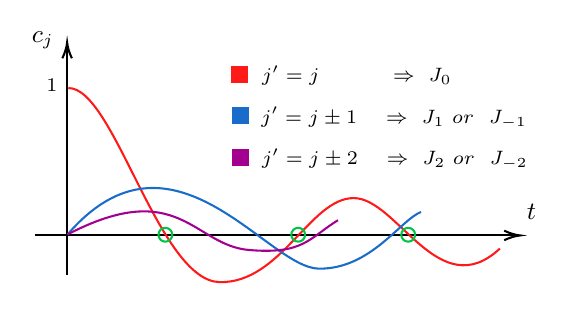
\begin{tikzpicture}[x=0.75pt,y=0.75pt,yscale=-1,xscale=1]
%uncomment if require: \path (0,130); %set diagram left start at 0, and has height of 130

%Straight Lines [id:da42292147954355674] 
\draw    (23,121) -- (23,11) ;
\draw [shift={(23,9)}, rotate = 90] [color={rgb, 255:red, 0; green, 0; blue, 0 }  ][line width=0.75]    (7.65,-2.3) .. controls (4.86,-0.97) and (2.31,-0.21) .. (0,0) .. controls (2.31,0.21) and (4.86,0.98) .. (7.65,2.3)   ;
%Straight Lines [id:da0938116227302922] 
\draw    (7.5,102) -- (239.25,102) ;
\draw [shift={(241.25,102)}, rotate = 180] [color={rgb, 255:red, 0; green, 0; blue, 0 }  ][line width=0.75]    (7.65,-2.3) .. controls (4.86,-0.97) and (2.31,-0.21) .. (0,0) .. controls (2.31,0.21) and (4.86,0.98) .. (7.65,2.3)   ;
%Curve Lines [id:da7388142079293656] 
\draw [color={rgb, 255:red, 255; green, 26; blue, 26 }  ,draw opacity=1 ]   (23.58,31) .. controls (45.58,30.5) and (67.08,124) .. (96.58,124.5) .. controls (126.08,125) and (140.08,84) .. (161.08,84) .. controls (182.08,84) and (202,135.83) .. (231.5,108.33) ;
%Curve Lines [id:da2797400644106053] 
\draw [color={rgb, 255:red, 25; green, 108; blue, 201 }  ,draw opacity=1 ]   (23.25,101.5) .. controls (73.75,43) and (119.33,117.67) .. (144.25,118) .. controls (169.17,118.33) and (183.5,94.67) .. (193.5,90.67) ;
%Curve Lines [id:da34662757016201506] 
\draw [color={rgb, 255:red, 163; green, 0; blue, 143 }  ,draw opacity=1 ]   (23.25,101.5) .. controls (76.83,73.67) and (83.83,106.67) .. (110.5,109) .. controls (137.17,111.33) and (139.83,103) .. (153.5,94.67) ;
%Shape: Circle [id:dp028498302535310938] 
\draw  [color={rgb, 255:red, 0; green, 196; blue, 69 }  ,draw opacity=1 ][line width=0.75]  (67,101.67) .. controls (67,99.83) and (68.49,98.33) .. (70.33,98.33) .. controls (72.17,98.33) and (73.67,99.83) .. (73.67,101.67) .. controls (73.67,103.51) and (72.17,105) .. (70.33,105) .. controls (68.49,105) and (67,103.51) .. (67,101.67) -- cycle ;
%Shape: Circle [id:dp30028872852521227] 
\draw  [color={rgb, 255:red, 0; green, 196; blue, 69 }  ,draw opacity=1 ][line width=0.75]  (131,101.67) .. controls (131,99.83) and (132.49,98.33) .. (134.33,98.33) .. controls (136.17,98.33) and (137.67,99.83) .. (137.67,101.67) .. controls (137.67,103.51) and (136.17,105) .. (134.33,105) .. controls (132.49,105) and (131,103.51) .. (131,101.67) -- cycle ;
%Shape: Circle [id:dp6051192164240733] 
\draw  [color={rgb, 255:red, 0; green, 196; blue, 69 }  ,draw opacity=1 ][line width=0.75]  (184,101.67) .. controls (184,99.83) and (185.49,98.33) .. (187.33,98.33) .. controls (189.17,98.33) and (190.67,99.83) .. (190.67,101.67) .. controls (190.67,103.51) and (189.17,105) .. (187.33,105) .. controls (185.49,105) and (184,103.51) .. (184,101.67) -- cycle ;
%Shape: Square [id:dp9109798777185496] 
\draw  [draw opacity=0][fill={rgb, 255:red, 255; green, 26; blue, 26 }  ,fill opacity=1 ] (102,20.33) -- (110.17,20.33) -- (110.17,28.5) -- (102,28.5) -- cycle ;
%Shape: Square [id:dp708254493093753] 
\draw  [draw opacity=0][fill={rgb, 255:red, 25; green, 108; blue, 201 }  ,fill opacity=1 ] (102.33,40.33) -- (110.5,40.33) -- (110.5,48.5) -- (102.33,48.5) -- cycle ;
%Shape: Square [id:dp732226894539835] 
\draw  [draw opacity=0][fill={rgb, 255:red, 163; green, 0; blue, 143 }  ,fill opacity=1 ] (102.67,60.33) -- (110.83,60.33) -- (110.83,68.5) -- (102.67,68.5) -- cycle ;

% Text Node
\draw (4.5,2.4) node [anchor=north west][inner sep=0.75pt]  [font=\small]  {$c_{j}$};
% Text Node
\draw (11.5,24.9) node [anchor=north west][inner sep=0.75pt]  [font=\scriptsize]  {$1$};
% Text Node
\draw (115.33,18.73) node [anchor=north west][inner sep=0.75pt]  [font=\scriptsize]  {$j'=j\ \ \ \ \ \ \ \ \ \Rightarrow \ J_{0}$};
% Text Node
\draw (115,38.73) node [anchor=north west][inner sep=0.75pt]  [font=\scriptsize]  {$j'=j\pm 1\ \ \ \Rightarrow \ J_{1} \ \text{or} \ \ J_{-1}$};
% Text Node
\draw (115.33,58.73) node [anchor=north west][inner sep=0.75pt]  [font=\scriptsize]  {$j'=j\pm 2\ \ \ \Rightarrow \ J_{2} \ \text{or} \ \ J_{-2}$};
% Text Node
\draw (243,85.4) node [anchor=north west][inner sep=0.75pt]  [font=\small]  {$t$};


\end{tikzpicture}
 }
\end{minipage}\hfill
\begin{minipage}{0.45\textwidth}
\begin{itemize}
    \item $c_{j}$ starts from $1$ (we prepared the system in this state) and then the particle starts spreading.
    \item For some time $t^*$ there exist null points of $c_j(t^*) = 0$. This is a destructive interference, nothing less than diffraction. This is why we can reproduce the same physics with purely optical systems.
\end{itemize}
\end{minipage}



\vspace{1em}

This concludes our discussion about single particle physics. Now we are ready to approach this topic from a many body perspective, i.e. many interacting atoms in a lattice.





\section{Interactions}

Materials are made by many interacting particles. For example, the interaction between electrons leads to superconductivity, ferromagnetism or insulators. These topics are usually studied in quantum many-body courses.

The simulations of many body systems are computationally challenging, because the dimension of the Hilbert spaces scales exponentially in the system size. For instance, a chain of $N_s$ spins implies that $dim(H_s) = 2^{N_s}$.\\

It is, at least computationally, an intractable problem. That is why most of the 20th century condenser matter physics has been devoted to develop methods, theoretical and (later) numerical, to address this problems, aiming to simplify the dimensionality of the problem.
\textbf{Analog quantum simulations} allow us to tackle the problem from another point of view, which is to deal with an target exponentially large Hilbert space using a system which is itself an exponentially large Hilbert space.
Analog quantum simulations are basically a mapping of a target problem to a real physical system.\\

\noindent This is a sufficient motivation to describe briefly the interactions and what kind of phenomena we can observe and model using algebraic models.

\vspace{1em}

Let us consider two atoms as dipoles (this is a rather classical way to solve the problem, since we know that atoms cannot have a permanent dipole).
The interaction potential between them is
\begin{equation*}
    V(\underbrace{\vec{r}_1-\vec{r}_2}_{\equiv\vec{r}}) = \frac{1}{4\pi\varepsilon_0r^3}
    \left[ \vec{d}_1\cdot \vec{d}_2 -3(\vec{d}_1\cdot\vec{r})(\vec{d}_2\cdot\vec{r})\right]
\end{equation*}

The scattering potential is complicated to solve, but for low $T$ (low energy) only the angular momentum $L=0$ is relevant (the centrifugal barrier inhibits the atom to scatter to larger angular momentum states). The angular momentum $\vec{L}$ is intended with respect to the relative coordinate $\vec{r}$.


\subsection{S-wave channel/scattering}

$L=0$ is usually called \textbf{S-wave channel} or scattering. It means basically that 
$$V(\vec{r}) \simeq u_0\delta^{(3)}(\vec{r}) \;\;.$$
Thinking of atoms as spheres, this approximation means that there is interaction only when the spheres overlap completely. We know it is not true, because there is a potential barrier that forbids the atoms to do so... instead, the atoms would ``touch" when their relative distance is some value $r^*>0$ (an ``effective bouncing radius").

Nevertheless, there exist some atoms that overlap, and they are bosonic atoms, like $\prescript{87}{}{Rb}$, $\prescript{27}{}{Na}$ and $\prescript{7}{}{Li}$.

We observe that combinations of an even number of fermions lead to bosonic wave-functions (spins would sum up to integer values $\Rightarrow$ Boson statistics).

In neutral atoms, the number of protons (it is made of three quarks, so it is a fermion) equals to the number of electrons. The number of fermions is even. The only way to discriminate is to count neutrons!

\noindent \textbf{Example} of Lithium: $Z_{Li} = 3$.
\begin{align*}
    \text{Neutrons}(\prescript{7}{}{Li}) = 7-Z_{Li} = 4 &\qquad \text{(even)} &\Rightarrow \text{boson}&&\\
    \text{Neutrons}(\prescript{6}{}{Li}) = 6-Z_{Li} = 3 &\qquad \text{(odd)} &\Rightarrow \text{fermion}&&
\end{align*}

\noindent What does this mean in terms of S-wave?
\begin{itemize}
    \item \textbf{Fermions} interact with S-Wave if the two atoms are in different internal states.
    \begin{equation*}
        (n_1, l_1, m_1, s_1)
        \neq (n_2, l_2, m_2, s_2)
    \end{equation*}
    Examples: $\prescript{6}{}{Li}$, $\prescript{40}{}{K}$, ...
    \item It is easier to describe \textbf{bosons}.

    We take the state $\psi_a(x)$ where $\alpha$ is a collection of quantum numbers $\alpha = (n, l, m)$ or another level of lattice physics (for example a Wannier function). The (most generic) wave-function of two atoms is symmetric for exchange of $r_i$:
    \begin{equation*}
        \Psi_{\alpha\beta}(\vec{r}_1,\vec{r}_2) = \frac{1}{2}
        \left[
            \psi_\alpha(\vec{r}_1)\psi_\beta(\vec{r}_2) +
            \psi_\alpha(\vec{r}_2)\psi_\beta(\vec{r}_1)
        \right]\delta_{\alpha\beta}
    \end{equation*}
    You may also have seen this in terms of the Slater determinant.
    
    The internal energy would be
    \begin{align*}
        E_{int} &= \int d\vec{r}_1 d\vec{r}_2
        \Psi^*(\vec{r}_1,\vec{r}_2) u_0 \delta(\vec{r}_1-\vec{r}_2) \Psi(\vec{r}_1,\vec{r}_2)\\
        % all the possibilities
        &= \frac{u_0}{4} \int d\vec{r}_1 d\vec{r}_2
        \left[
            \psi(\vec{r}_1)\psi(\vec{r}_2)\psi(\vec{r}_1)\psi(\vec{r}_2) + ... + \psi(\vec{r}_2)\psi(\vec{r}_1)\psi(\vec{r}_2)\psi(\vec{r}_1)
        \right] \delta(\vec{r}_1 - \vec{r}_2)\\
        &= \frac{u_0}{4} \int d\vec{r}_1 d\vec{r}_2 \cdot
            4 |\psi(\vec{r}_1)|^2|\psi(\vec{r}_2)|^2
            \delta(\vec{r}_1 - \vec{r}_2)\\
        &= u_0 \int d\vec{r}_1 |\psi(\vec{r}_1)|^4 =
            u_0 \int dr |\psi(r)|^4 \equiv U
    \end{align*}
    
    Thus, if we know the wave-functions then we know the energy of interaction. If we had Wannier functions, we could also write
    \begin{equation*}
    \Rightarrow \bra{w(x_j)w(x_{j'})} \hat{V}_{int} \ket{w(x_j)w(x_{j'})} = \delta_{j,j'}U
    \end{equation*}


\end{itemize}







% LECTURE 26 (20 jan)

\section{Quantum phase transitions}

In this section we will review two models featuring quantum phase transitions, with a particular focus on a quantum phase transition from superfluid to Mott insulator observed with ultra-cold atoms\footnote{\href{https://www.nature.com/articles/415039aa}{Greiner, M., Mandel, O., Esslinger, T. et al. Quantum phase transition from a superfluid to a Mott insulator in a gas of ultracold atoms - Nature 415, 39–44 (2002)}}.





\subsection{Bose-Hubbard model}

Let us consider a system of $N$ bosons hopping on a $N_s$ sites lattice (with hopping parameter $J$) and interacting when close enough.

We need some more formalism to address this problem properly. To take a shortcut, we just say that, like for photons, the Wannier functions $\ket{j}\equiv\ket{w_j}$ can be written in terms of creation/destruction operators (satisfying the harmonic oscillator commutation rules)
$$ \left[\hat{a}_j, \hat{a}_{j'}^\dag\right] = \delta_{j,j'}
   \qquad
   \left[\hat{a}_j, \hat{a}_{j'}\right] =
   \left[\hat{a}_j, \hat{a}_{j'}^\dag\right] = 0
$$
which create/destroy bosons in a Wannier function mode. Every particle is a quantum field! Thus, the hopping Hamiltonian can be rewritten as
\begin{align*}
\hat{H}_{hop} &= -J\sum_j
    \left( \ket{j+1}\bra{j} + h.c. \right) =\\
&= -J\sum_j
    \left( \hat{a}_{j+1}^\dag\hat{a}_{j} + \hat{a}_{j}^\dag\hat{a}_{j+1} \right)
\end{align*}

Now we want to write the interaction part $\hat{H}_{\text{int}}$. Also in this case, the Hilbert space is similar to the one with photons on mode $j$. Instead of counting photons, we count the number of bosons in each mode (Wannier function) $\ket{w_j}$:
\begin{equation*}
    \ket{n_{j=1}} \otimes \ket{n_{j=2}} \otimes ... \otimes \ket{n_{j=1}} \otimes ...
\end{equation*}
We have previously seen that the energy of two atoms in the same orbital is $U$. Now we want to find an hamiltonian that returns $U$ when it is contracted with a state with two particles in the same mode, and return zero for states with just one particle.

We do not prove it in a rigorous way, but we will see that the following hamiltonian  satisfies our requests
\begin{equation*}
    \hat{H}_{int} = \frac{U}{2}\sum_j \hat{n}_j (\hat{n}_j-1)  \qquad\qquad \text{where }\;\; \hat{n}_j = \hat{a}_j^\dag \hat{a}_j
\end{equation*}

\noindent Let us check the quantity $\bra{\psi}\hat{H}_{int}\ket{\psi}$ for...
\begin{itemize}
    \item ...\emph{2 particles}: $\ket{\psi} = \ket{0}\otimes ...\otimes\ket{0}\otimes\ket{2_j}\otimes\ket{0}\otimes ...$\\
    $$\begin{cases}
        \hat{H}_{int}^{(j)} \ket{0_j} = \frac{U}{2}0(0-1)\ket{0_j} = 0\ket{0_j}\\
        \hat{H}_{int}^{(j)} \ket{2_j} = \frac{U}{2}2(2-1)\ket{2_j} = U\ket{2_j}
    \end{cases} \Rightarrow \bra{\psi}\hat{H}_{int}\ket{\psi} = U = E_{int}$$
    \item ...\emph{1 particle}: $\ket{\psi} = \ket{0}\otimes ...\otimes\ket{0}\otimes\ket{1_j}\otimes\ket{0}\otimes ...$\\
    \begin{equation}
    \label{eq:bh-interaction-min}
    \begin{cases}
        \hat{H}_{int}^{(j)} \ket{0_j} = \frac{U}{2}0(0-1) \ket{0_j} = 0\ket{0_j}\\
        \hat{H}_{int}^{(j)} \ket{2_j} = \frac{U}{2}1(1-1) \ket{2_j} = 0\ket{1_j}
    \end{cases}
    \Rightarrow  \bra{\psi}\hat{H}_{int}\ket{\psi} = 0
    \end{equation}\\
    The interaction energy is zero because one particle is not interacting with any other one.
\end{itemize}


The total hamiltonian for the Bose-Hubbard model is
\begin{equation}
    \hat{H} = -J\sum_j\left(
        \hat{a}_{j+1}^\dag\hat{a}_{j} + \hat{a}_{j}^\dag\hat{a}_{j+1}
    \right) + \frac{U}{2} \sum_j \hat{n}_{j}(\hat{n}_{j}-1)
\end{equation}
%
The problem is that the basis we have chosen do not diagonalize both terms at the same time: $\left[\hat{H}_{hop}, \hat{H}_{int}\right] \neq 0$. Diagonalize $\hat{H}$ is hard: in principle there could be a basis, but no one has found it so far. There is no exact numerical solution either. That is why it would be nice to simulate this model on quantum hardware!\\

The Bose-Hubbard model has a phase transition which we can predict in an approximate way. Let us look at some particular cases:
\begin{itemize}

    \item For $U=0$ we neglect the interaction term. With a single particle, the spectrum is given by Eq. \ref{eq:spectrum-tight-binding} and we have approximated it to the first term ($\mu=1$).

    \begin{center}
        \scalebox{1}{ 

\tikzset{every picture/.style={line width=0.75pt}} %set default line width to 0.75pt        

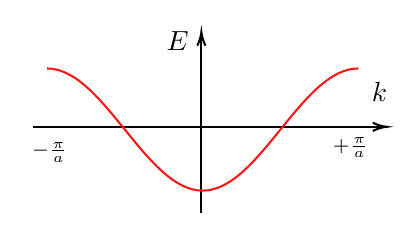
\begin{tikzpicture}[x=0.75pt,y=0.75pt,yscale=-1,xscale=1]
%uncomment if require: \path (0,104); %set diagram left start at 0, and has height of 104

%Straight Lines [id:da8978232046797772] 
\draw    (84.4,96.21) -- (84.4,11.2) ;
\draw [shift={(84.4,9.2)}, rotate = 90] [color={rgb, 255:red, 0; green, 0; blue, 0 }  ][line width=0.75]    (6.56,-1.97) .. controls (4.17,-0.84) and (1.99,-0.18) .. (0,0) .. controls (1.99,0.18) and (4.17,0.84) .. (6.56,1.97)   ;
%Straight Lines [id:da7309963691958787] 
\draw    (3.5,54.86) -- (171.57,54.86) ;
\draw [shift={(173.57,54.86)}, rotate = 180] [color={rgb, 255:red, 0; green, 0; blue, 0 }  ][line width=0.75]    (6.56,-1.97) .. controls (4.17,-0.84) and (1.99,-0.18) .. (0,0) .. controls (1.99,0.18) and (4.17,0.84) .. (6.56,1.97)   ;
%Shape: Wave [id:dp933616384096774] 
\draw  [color={rgb, 255:red, 255; green, 21; blue, 21 }  ,draw opacity=1 ] (10,26.74) .. controls (23.57,26.74) and (35.27,41.1) .. (47.5,56.17) .. controls (59.73,71.25) and (71.43,85.6) .. (85,85.6) .. controls (98.57,85.6) and (110.27,71.25) .. (122.5,56.17) .. controls (134.73,41.1) and (146.43,26.74) .. (160,26.74) ;

% Text Node
\draw (165,32.13) node [anchor=north west][inner sep=0.75pt]  [font=\normalsize]  {$k$};
% Text Node
\draw (66.19,7.59) node [anchor=north west][inner sep=0.75pt]  [font=\normalsize]  {$E$};
% Text Node
\draw (1.21,60.83) node [anchor=north west][inner sep=0.75pt]  [font=\scriptsize]  {$-\frac{\pi }{a}$};
% Text Node
\draw (146.3,58.6) node [anchor=north west][inner sep=0.75pt]  [font=\scriptsize]  {$+\frac{\pi }{a}$};

\end{tikzpicture} }
    \end{center}
    
    The single particle ground state is the one with $k=0$, therefore we can write the single particle ground state as $\ket{GS}=a^\dag_{k=0}\ket{0}$. For N bosons, the expression easily generalizes to
    $$\ket{GS} = \left(\hat{a}^\dag_{k=0}\right)^{N}\ket{0} \;\;.$$ % normalization factor wrong in lecture notes?
    This is called Bose Einstein Condensate (BEC) and it has energy
    $$E_{BEC} = -2J \cos(ka)\big|_{k=0}\cdot N = -2J\cdot N$$

    The state we have constructed has a very nice property. Using a Fourier transform, one can write
    $$\hat{a}^\dag_k = \frac{1}{\sqrt{N_s}}\sum_j^{N_s} \hat{a}^\dag_j e^{ikja}$$
    but imposing $k=0$ and computing the polynomial expansion we get that
    \begin{align*}
        \ket{GS} &\propto
            \left( \hat{a}_1^\dag + \hat{a}_2^\dag  + ... + \hat{a}_{N_s}^\dag\right)^N \ket{0}
        = (\hat{a}_1^\dag)^N\ket{0} + (\hat{a}_1^\dag)^{N-1}\hat{a}_2\ket{0} + ...
    \end{align*}
    which means that all bosons are maximally delocalized with probability $\sim 1/N$ to be found on an arbitrary lattice site. Equivalently, we say that the GS (at momentum 0) is a superposition of states in which the (average) number of particles on site $j$ is not fixed. The system is said to be in the \textbf{superfluid state} (for a free Bose gas). Also, it is
    $$\psi_j \equiv \bra{GS}\hat{a}_j\ket{GS}  \neq 0$$
    This behavior reminds us of photons in coherent states!
    It can be proven with thermodynamic theory that this state is a coherent state for many particles.
    
    \item Now we can look at the case $J\ll U$, which is the regime of dominating interactions. We set $U>0$ because of repulsive interaction. To find the ground state, we have to minimize the interaction energy. We have seen in Eq. \ref{eq:bh-interaction-min} that with only one particle in a site the interaction energy is exactly zero and that the energy increases when particles are packed together. Thus, the minimum value of the energy (zero) is achieved with one particle per site
    $$\ket{GS} = \ket{1_{j=1}}\otimes\ket{1_{j=2}}\otimes...\otimes\ket{1_{j=N_s}} = \prod_{j=1}^{N_s}\hat{a}_j^\dag\ket{0}$$
    \begin{center}
        \scalebox{1.2}{
            

\tikzset{every picture/.style={line width=0.75pt}} %set default line width to 0.75pt        

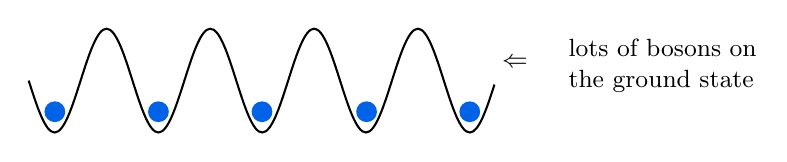
\begin{tikzpicture}[x=0.75pt,y=0.75pt,yscale=-1,xscale=1]
%uncomment if require: \path (0,67); %set diagram left start at 0, and has height of 67

%Shape: Wave [id:dp49770649258615707] 
\draw  [color={rgb, 255:red, 0; green, 0; blue, 0 }  ,draw opacity=1 ] (10,35) .. controls (14.08,47.81) and (17.98,60) .. (22.5,60) .. controls (27.02,60) and (30.92,47.81) .. (35,35) .. controls (39.08,22.19) and (42.98,10) .. (47.5,10) .. controls (52.02,10) and (55.92,22.19) .. (60,35) .. controls (64.08,47.81) and (67.98,60) .. (72.5,60) .. controls (77.02,60) and (80.92,47.81) .. (85,35) .. controls (89.08,22.19) and (92.98,10) .. (97.5,10) .. controls (102.02,10) and (105.92,22.19) .. (110,35) .. controls (114.08,47.81) and (117.98,60) .. (122.5,60) .. controls (127.02,60) and (130.92,47.81) .. (135,35) .. controls (139.08,22.19) and (142.98,10) .. (147.5,10) .. controls (152.02,10) and (155.92,22.19) .. (160,35) .. controls (164.08,47.81) and (167.98,60) .. (172.5,60) .. controls (177.02,60) and (180.92,47.81) .. (185,35) .. controls (189.08,22.19) and (192.98,10) .. (197.5,10) .. controls (202.02,10) and (205.92,22.19) .. (210,35) .. controls (214.08,47.81) and (217.98,60) .. (222.5,60) .. controls (226.8,60) and (230.54,48.98) .. (234.4,36.88) ;
%Shape: Circle [id:dp870205875238355] 
\draw  [draw opacity=0][fill={rgb, 255:red, 0; green, 98; blue, 230 }  ,fill opacity=1 ] (17.6,50) .. controls (17.6,47.24) and (19.84,45) .. (22.6,45) .. controls (25.36,45) and (27.6,47.24) .. (27.6,50) .. controls (27.6,52.76) and (25.36,55) .. (22.6,55) .. controls (19.84,55) and (17.6,52.76) .. (17.6,50) -- cycle ;
%Shape: Circle [id:dp7879328877360514] 
\draw  [draw opacity=0][fill={rgb, 255:red, 0; green, 98; blue, 230 }  ,fill opacity=1 ] (67.5,50) .. controls (67.5,47.24) and (69.74,45) .. (72.5,45) .. controls (75.26,45) and (77.5,47.24) .. (77.5,50) .. controls (77.5,52.76) and (75.26,55) .. (72.5,55) .. controls (69.74,55) and (67.5,52.76) .. (67.5,50) -- cycle ;
%Shape: Circle [id:dp676964482149583] 
\draw  [draw opacity=0][fill={rgb, 255:red, 0; green, 98; blue, 230 }  ,fill opacity=1 ] (117.4,50) .. controls (117.4,47.24) and (119.64,45) .. (122.4,45) .. controls (125.16,45) and (127.4,47.24) .. (127.4,50) .. controls (127.4,52.76) and (125.16,55) .. (122.4,55) .. controls (119.64,55) and (117.4,52.76) .. (117.4,50) -- cycle ;
%Shape: Circle [id:dp5468116419516752] 
\draw  [draw opacity=0][fill={rgb, 255:red, 0; green, 98; blue, 230 }  ,fill opacity=1 ] (167.8,50) .. controls (167.8,47.24) and (170.04,45) .. (172.8,45) .. controls (175.56,45) and (177.8,47.24) .. (177.8,50) .. controls (177.8,52.76) and (175.56,55) .. (172.8,55) .. controls (170.04,55) and (167.8,52.76) .. (167.8,50) -- cycle ;
%Shape: Circle [id:dp3355085376283945] 
\draw  [draw opacity=0][fill={rgb, 255:red, 0; green, 98; blue, 230 }  ,fill opacity=1 ] (217.5,50) .. controls (217.5,47.24) and (219.74,45) .. (222.5,45) .. controls (225.26,45) and (227.5,47.24) .. (227.5,50) .. controls (227.5,52.76) and (225.26,55) .. (222.5,55) .. controls (219.74,55) and (217.5,52.76) .. (217.5,50) -- cycle ;

% Text Node
\draw (236.6,22.85) node [anchor=north west][inner sep=0.75pt]  [font=\small]  {$\Leftarrow $};
% Text Node
\draw (268.6,13.65) node [anchor=north west][inner sep=0.75pt]  [font=\small] [align=left] {lots of bosons on\\the ground state};


\end{tikzpicture}

        }
    \end{center}
    and this ground state is unique.

    Since we have a fixed number of particles on each site and no fluctuation is allowed, we call this state \textbf{Mott-insulator phase}.
    $$\bra{GS}\hat{a}_j\ket{GS} \equiv \psi_j = 0$$

    If one wants to slightly change the number of particles of the GS, he would have to pay some energy $U$. Therefore, we say that in the Mott insulator there is an energy gap (difference in energy between the ground state and the first excite state) given by $U$.
    
\end{itemize}


\begin{tcolorbox}[breakable, enhanced]
\textbf{Recap}\\

    To rephrase the content of this section, let me quote the paper \href{https://www.nature.com/articles/415039aa}{Greiner, M., Mandel, O., Esslinger, T. et al. Quantum phase transition from a superfluid to a Mott insulator in a gas of ultracold atoms - Nature 415, 39–44 (2002)}.\\
    
    1) In the limit where the tunnelling term dominates the hamiltonian, the ground-state energy is minimized if the single-particle wavefunctions of $N$ atoms are spread out over the entire lattice with $N_s$ lattice sites. The many-body ground state (for a homogeneous system) is then given by:
    \[
    \ket{\psi}\propto \left(\sum_i^{N_s}\hat{a}_i^\dag\right)^N \ket{0}
    \]
    Here all atoms occupy the identical extended Bloch state. An important feature of this state is that the probability distribution for the local occupation $n_i$ of atoms on a single lattice site is poissonian, that is, its variance is given by $\text{Var}(n_i) =\langle n_i\rangle$. Furthermore, this state is well described by a macroscopic wavefunction with long-range phase coherence throughout the lattice.\\

    2) If interactions dominate the hamiltonian, the fluctuations in atom number become energetically very costly and the ground state of the system will instead consist of localized atomic wavefunctions with a fixed number of atoms per site that minimize the interaction energy. The many-body ground state is then a product of local Fock states for each lattice site. In this limit, the ground state of the many-body system for a commensurate filling of $n$ atoms per lattice site in the homogeneous case is given by
    \[
    \ket{\psi}\propto \prod_i^{N_s}(\hat{a}_i^\dag)^n\ket{0} 
    \]
    This Mott insulator state cannot be described by a macroscopic wavefunction like in a Bose condensed phase, and thus is not amenable to a treatment via the Gross-Pitaevskii equation or Bogoliubov's theory of weakly interacting bosons. In this state no phase coherence is prevalent in the system, but perfect correlations in the atom number exist between lattice sites.
\end{tcolorbox}



Right now we are looking at ``strange" ground levels that are not acting like ground states in intermediate conditions. Namely, we are looking for ground states, as function of $J/U$ in which the behavior changes:
\begin{center}
        \scalebox{1.2}{
            

\tikzset{every picture/.style={line width=0.75pt}} %set default line width to 0.75pt        

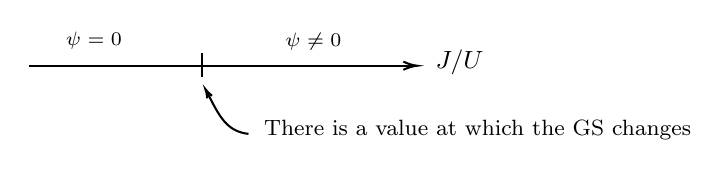
\begin{tikzpicture}[x=0.75pt,y=0.75pt,yscale=-1,xscale=1]
%uncomment if require: \path (0,75); %set diagram left start at 0, and has height of 75

%Straight Lines [id:da7677509231373215] 
\draw    (10.5,26.86) -- (195.57,26.86) ;
\draw [shift={(197.57,26.86)}, rotate = 180] [color={rgb, 255:red, 0; green, 0; blue, 0 }  ][line width=0.75]    (6.56,-1.97) .. controls (4.17,-0.84) and (1.99,-0.18) .. (0,0) .. controls (1.99,0.18) and (4.17,0.84) .. (6.56,1.97)   ;
%Straight Lines [id:da3257796010864502] 
\draw    (94,20.9) -- (94,32.1) ;
%Curve Lines [id:da5122812185238221] 
\draw    (116.4,59.7) .. controls (105.38,58.56) and (101.94,50.2) .. (96.48,39.76) ;
\draw [shift={(95.6,38.1)}, rotate = 61.82] [color={rgb, 255:red, 0; green, 0; blue, 0 }  ][line width=0.75]    (4.37,-1.32) .. controls (2.78,-0.56) and (1.32,-0.12) .. (0,0) .. controls (1.32,0.12) and (2.78,0.56) .. (4.37,1.32)   ;

% Text Node
\draw (205,17.63) node [anchor=north west][inner sep=0.75pt]  [font=\small]  {$J/U$};
% Text Node
\draw (26.91,9.03) node [anchor=north west][inner sep=0.75pt]  [font=\scriptsize]  {$\psi =0$};
% Text Node
\draw (132.71,9.43) node [anchor=north west][inner sep=0.75pt]  [font=\scriptsize]  {$\psi \neq 0$};
% Text Node
\draw (122.4,51.8) node [anchor=north west][inner sep=0.75pt]  [font=\footnotesize] [align=left] {There is a value at which the GS changes};


\end{tikzpicture}

        }
\end{center}






\subsection{1D Ising model}

Let us discuss another model which features phase transitions: the Ising model.
We consider the following interaction hamiltonian
\begin{equation}
\label{eq:ising}
\hat{H}=-J\sum_{i,j} \hat{S_i^z}\hat{S_j^z}
\end{equation}
We also define the magnetization $M$ as the ensemble average of all the spins
$$M \equiv \frac{1}{N_s} \sum_i\langle \hat{S}_i^z\rangle$$

What is the GS of Eq. \ref{eq:ising} as a function of the temperature $T$? We expect that the energy is minimized when $T=0$, so that all the spins are aligned in the same direction (if $J>0$). In this settings, the magnetization would also achieve its maximum value: $M(T=0) = 1$.


When one increases the temperature $T$, the spins interact with each other and are allowed to flip. It can be proven that there exists a critical value $T_c$ for which the magnetization is lost $M(T_c)=0$, and this happens the spins are in a superposition of all the possible configurations.
\begin{center}
    \scalebox{1.2}{ 

\tikzset{every picture/.style={line width=0.75pt}} %set default line width to 0.75pt        

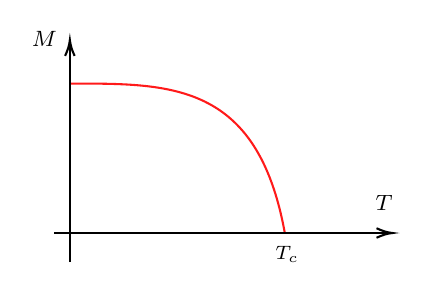
\begin{tikzpicture}[x=0.75pt,y=0.75pt,yscale=-1,xscale=1]
%uncomment if require: \path (0,130); %set diagram left start at 0, and has height of 130

%Curve Lines [id:da5736115837190213] 
\draw [color={rgb, 255:red, 255; green, 26; blue, 26 }  ,draw opacity=1 ]   (22.83,30) .. controls (71.17,30) and (113.17,29) .. (126.5,101.67) ;
%Straight Lines [id:da7029677561387601] 
\draw    (23,116) -- (23,11) ;
\draw [shift={(23,9)}, rotate = 90] [color={rgb, 255:red, 0; green, 0; blue, 0 }  ][line width=0.75]    (7.65,-2.3) .. controls (4.86,-0.97) and (2.31,-0.21) .. (0,0) .. controls (2.31,0.21) and (4.86,0.98) .. (7.65,2.3)   ;
%Straight Lines [id:da09730999984454025] 
\draw    (15.5,102) -- (176.4,102) ;
\draw [shift={(178.4,102)}, rotate = 180] [color={rgb, 255:red, 0; green, 0; blue, 0 }  ][line width=0.75]    (7.65,-2.3) .. controls (4.86,-0.97) and (2.31,-0.21) .. (0,0) .. controls (2.31,0.21) and (4.86,0.98) .. (7.65,2.3)   ;

% Text Node
\draw (3.17,3.57) node [anchor=north west][inner sep=0.75pt]  [font=\footnotesize]  {$M$};
% Text Node
\draw (168.87,82.4) node [anchor=north west][inner sep=0.75pt]  [font=\footnotesize]  {$T$};
% Text Node
\draw (120.52,107.02) node [anchor=north west][inner sep=0.75pt]  [font=\scriptsize]  {$T_{c}$};


\end{tikzpicture}
 }
\end{center}

The critical temperature $T_c$ can be computed from the partition function (if one has written it right from the beginning). Another approach is to consider the Landau free energy.

The Landau free energy functional is an analytic function of a suitable order parameter; for this system we notice that the magnetization $M$ is small enough around the critical temperature, thus it can be used as an order parameter:
$$F_L(T)\big|_{T\simeq T_c} = a_0(T) + a_2(T)M^2 + a_4(T)M^4 + \dots \qquad M\rightarrow0$$
In practice we have expanded $F_L$ as a Taylor series. The free energy will only be a function of even powers of the order parameter, because of symmetries of our system. Then, one minimizes the free energy with the zeros of the partial derivative:
\begin{equation*}
    \Rightarrow 0 = \frac{\partial F_L}{\partial M} = 2 a_2 M + 4 a_4 M^3 = 2M(a_2 + 2a_4 M^2)
\end{equation*}
and we find the minimum at $M=0$ or $M_{\pm}=\pm\sqrt{-\frac{a_2}{2a_4}}$.


For the system to be thermodynamically stable (that is, the system does not seek an infinite order parameter to minimize the energy), the coefficient of the highest even power of the order parameter must be positive, so $a_4(T)>0$. For simplicity, one can assume that $a_4(T)|_{T\simeq T_c} = a_4^* >0$, a constant, near the critical temperature. Furthermore, since $a_2$ changes sign above and below the critical temperature, one can expand $a_2(T)|_{T\simeq T_c} \simeq a_2^*(T-T_C)$, where it is assumed that \begin{itemize}
    \item for $T>T_c \Rightarrow a_2(T)>0 \qquad \Rightarrow M=0$ \;\; ($M_\pm \notin \mathbb{R}$, it does not exist)
    \item for $T<T_c \Rightarrow a_2(T)<0 \qquad \Rightarrow M=M_\pm$
\end{itemize}


\begin{center}
    \scalebox{1.2}{ 

\tikzset{every picture/.style={line width=0.75pt}} %set default line width to 0.75pt        

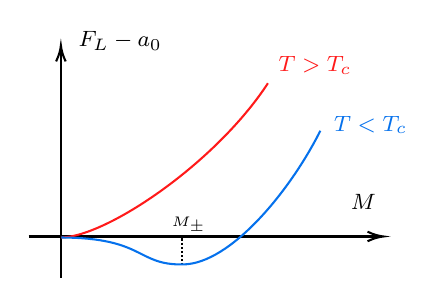
\begin{tikzpicture}[x=0.75pt,y=0.75pt,yscale=-1,xscale=1]
%uncomment if require: \path (0,130); %set diagram left start at 0, and has height of 130

%Straight Lines [id:da16333278826217945] 
\draw  [dash pattern={on 0.75pt off 0.75pt}]  (81.26,101.95) -- (81.26,114.52) ;
%Straight Lines [id:da19867223914819143] 
\draw    (23,121) -- (23,11) ;
\draw [shift={(23,9)}, rotate = 90] [color={rgb, 255:red, 0; green, 0; blue, 0 }  ][line width=0.75]    (7.65,-2.3) .. controls (4.86,-0.97) and (2.31,-0.21) .. (0,0) .. controls (2.31,0.21) and (4.86,0.98) .. (7.65,2.3)   ;
%Straight Lines [id:da11391700401294191] 
\draw    (7.5,101) -- (176.4,101) ;
\draw [shift={(178.4,101)}, rotate = 180] [color={rgb, 255:red, 0; green, 0; blue, 0 }  ][line width=0.75]    (7.65,-2.3) .. controls (4.86,-0.97) and (2.31,-0.21) .. (0,0) .. controls (2.31,0.21) and (4.86,0.98) .. (7.65,2.3)   ;
%Curve Lines [id:da6293915069092999] 
\draw [color={rgb, 255:red, 255; green, 26; blue, 26 }  ,draw opacity=1 ]   (23.25,101.5) .. controls (45.25,101) and (97.6,65.67) .. (122.75,27.17) ;
%Curve Lines [id:da5951789274075004] 
\draw [color={rgb, 255:red, 5; green, 113; blue, 236 }  ,draw opacity=1 ]   (23.25,101.5) .. controls (63.75,101.67) and (59.2,114.87) .. (82,114.47) .. controls (104.8,114.07) and (133.6,78.87) .. (148,50.07) ;

% Text Node
\draw (30.0,0.9) node [anchor=north west][inner sep=0.75pt]  [font=\footnotesize]  {$F_{L} - a_0$};
% Text Node
\draw (161.2,79.4) node [anchor=north west][inner sep=0.75pt]  [font=\footnotesize]  {$M$};
% Text Node
\draw (126.4,12.93) node [anchor=north west][inner sep=0.75pt]  [font=\footnotesize,color={rgb, 255:red, 255; green, 26; blue, 26 }  ,opacity=1 ]  {$T >T_{c}$};
% Text Node
\draw (153.2,41.4) node [anchor=north west][inner sep=0.75pt]  [font=\footnotesize,color={rgb, 255:red, 5; green, 113; blue, 236 }  ,opacity=1 ]  {$T< T_{c}$};
% Text Node
\draw (74.86,90.02) node [anchor=north west][inner sep=0.75pt]  [font=\tiny]  {$M_{\pm }$};


\end{tikzpicture}

 }
\end{center}

The value for which $a_2(T)=0$ allows to identify the phase transition. Is this accurate? We will not investigate this further...

Transitions which occur controlling a finite value temperature $T_c>0$ are called \emph{Classical Phase Transitions}. Instead, a \textbf{Quantum Phase Transition} (QPT) can only be accessed by varying a physical parameter (such as magnetic field or pressure) at absolute zero temperature $T=0$.\\




\subsection{Perturbation theory to calculate the energy of Bose-Hubbard model}

Let us change the parameter $T$ to $J/U$. The free energy is now
$F=E(T) - T S(T)$.\\
% E(T) = energy, T = temperature, S(T) = entropy
%
More specifically, at $T=0 \Rightarrow F = E(T=0)$. Thus, the ground state energy $E_{GS}$ is a function of the order parameter $\psi_j$ and $J/U$ (called control parameter)
\begin{equation}
    E_{GS} \simeq E_0 + a_2(J/U)\psi^2 + a_4(J/U)\psi^4
    \qquad
    \psi_j \equiv \bra{GS}\hat{a}_j\ket{GS}
    \label{eq:landau-bh}
\end{equation}
We want to find the $J/U$ for which there is the phase transition. \textbf{We will address this problem using a perturbation method}. We start from the BH model
\begin{equation*}
    \hat{H} = -J\sum_j\left(
        \hat{a}_{j+1}^\dag\hat{a}_{j} +
        \hat{a}_{j}^\dag\hat{a}_{j+1}
    \right) + \frac{U}{2}\sum_j \hat{n}_j(\hat{n}_j-1)
\end{equation*}

But if $\ket{GS}$ is approximately behaving as a coherent state with some quantum fluctuation, then from the point of view of matrix elements we could write that $$\hat{a}_j = \underbrace{\bra{GS}\hat{a}_j\ket{GS}}_{\psi_j} \;\; + \underbrace{\delta\hat{a}_j}_{\mathclap{\text{small fluctuation}}}$$
(in the same fashion we did for the electric field: $\hat{E} = \langle\hat{E}\rangle + \Delta E$).

\noindent If we also impose translational invariance over the sites $j$ (all the sites are equivalent), then $\psi_j$ does not depend on the site ($\psi_j = \psi = \text{const}$). We can also redefine the phase of the operators ($\hat{a}_j$) to impose $\psi^*=\psi$. Therefore
\begin{align*}
    \hat{a}^\dag_j\hat{a}_{j+1} &= 
        (\psi + \delta \hat{a}^\dag_{j})(\psi + \delta \hat{a}_{j+1})
    = \psi^2 + \psi \delta \hat{a}_{j+1} + \psi\delta \hat{a}^\dag_{j} + \underbrace{\delta \hat{a}^\dag_{j}\delta \hat{a}_{j+1}}_{\text{small}}= \\
    &\equalexpl{back to previous picture} \psi^2 + \psi(\hat{a}^\dag_{j}-\psi) + \psi(\hat{a}_{j+1} - \psi) =\\
    &= -\psi^2 + \psi(\hat{a}^\dag_{j} + \hat{a}_{j+1})
\end{align*}

\noindent Accounting for the hermitian conjugate an summing all up, we get
\begin{equation*}
    (\hat{a}^\dag_{j}\hat{a}_{j+1} + h.c.) \simeq -2\psi^2 + \psi(\hat{a}^\dag_{j}+\hat{a}_{j+1}+\hat{a}_{j}+\hat{a}^\dag_{j+1})
\end{equation*}
\begin{equation*}
    \Rightarrow \sum_j (\hat{a}^\dag_{j}\hat{a}_{j+1} + h.c.) \simeq -2N_s\psi^2 + 2\psi\sum_j(\hat{a}^\dag_{j}+\hat{a}_{j})
\end{equation*}
where we have $N_s$ instead of $(N_s-1)$ because of the periodic boundary conditions.

\begin{equation}
    \hat{H} \simeq 
        \underbrace{-2J\psi\sum_j(\hat{a}^\dag_{j}+\hat{a}_{j}) + 2JN_s\psi^2}_{\text{approximated hopping term} \;\;\equiv \hat{V}(\psi)}
    + \underbrace{\frac{U}{2}\sum_j \hat{n}_j(\hat{n}_j-1)}_{\text{no approximation}\;\; \equiv \hat{H}_0}
\end{equation}

\noindent In this machinery, we have approximated only the hopping term, which now is a perturbation $\hat{V}$ with small parameter $\psi$ (up to second order). The second term is not approximated, so we will consider it to be the unperturbed hamiltonian $\hat{H_0}$. However, we have renounced to particle conservation! This means that to remain rigorous we have to control the particle number $N$, for instance using a chemical potential $-\mu\hat{N}$ (in statistical mechanics $\mu$ fixes the average number of particles).\\


In perturbation theory
$$E_{GS} = E_g + \bra{g}\hat{V}\ket{g} + \sum_{e\neq g}\frac{|\bra{e}\hat{V}\ket{g}|^2}{E_g-E}$$

\noindent The ground state of $\hat{H}_0 = \frac{U}{2}\sum_j \hat{n}_j(\hat{n}_j-1) - \mu \sum_j\hat{n}_j$ is $\ket{g}=\ket{1}\otimes...\otimes\ket{1}$, so
    \begin{equation*}
        E_g = -\mu N_s  \qquad\qquad \text{and} \qquad \langle \hat{N} \rangle = N_s
    \end{equation*}

\noindent For excited states, we consider either $\ket{e_+}$ or $\ket{e_-}$:
\begin{enumerate}
    \item $\ket{e_+}$ (has all 1s except for a 2)
    \begin{center}
        \scalebox{1.2}{
            

\tikzset{every picture/.style={line width=0.75pt}} %set default line width to 0.75pt        

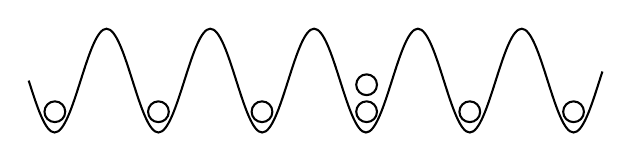
\begin{tikzpicture}[x=0.75pt,y=0.75pt,yscale=-1,xscale=1]
%uncomment if require: \path (0,67); %set diagram left start at 0, and has height of 67

%Shape: Wave [id:dp1825623717070861] 
\draw  [color={rgb, 255:red, 0; green, 0; blue, 0 }  ,draw opacity=1 ] (10,35) .. controls (14.08,47.81) and (17.98,60) .. (22.5,60) .. controls (27.02,60) and (30.92,47.81) .. (35,35) .. controls (39.08,22.19) and (42.98,10) .. (47.5,10) .. controls (52.02,10) and (55.92,22.19) .. (60,35) .. controls (64.08,47.81) and (67.98,60) .. (72.5,60) .. controls (77.02,60) and (80.92,47.81) .. (85,35) .. controls (89.08,22.19) and (92.98,10) .. (97.5,10) .. controls (102.02,10) and (105.92,22.19) .. (110,35) .. controls (114.08,47.81) and (117.98,60) .. (122.5,60) .. controls (127.02,60) and (130.92,47.81) .. (135,35) .. controls (139.08,22.19) and (142.98,10) .. (147.5,10) .. controls (152.02,10) and (155.92,22.19) .. (160,35) .. controls (164.08,47.81) and (167.98,60) .. (172.5,60) .. controls (177.02,60) and (180.92,47.81) .. (185,35) .. controls (189.08,22.19) and (192.98,10) .. (197.5,10) .. controls (202.02,10) and (205.92,22.19) .. (210,35) .. controls (214.08,47.81) and (217.98,60) .. (222.5,60) .. controls (227.02,60) and (230.92,47.81) .. (235,35) .. controls (239.08,22.19) and (242.98,10) .. (247.5,10) .. controls (252.02,10) and (255.92,22.19) .. (260,35) .. controls (264.08,47.81) and (267.98,60) .. (272.5,60) .. controls (277.02,60) and (280.92,47.81) .. (285,35) .. controls (285.47,33.53) and (285.93,32.06) .. (286.4,30.63) ;
%Shape: Circle [id:dp707885383803819] 
\draw  [color={rgb, 255:red, 0; green, 0; blue, 0 }  ,draw opacity=1 ] (17.6,50) .. controls (17.6,47.24) and (19.84,45) .. (22.6,45) .. controls (25.36,45) and (27.6,47.24) .. (27.6,50) .. controls (27.6,52.76) and (25.36,55) .. (22.6,55) .. controls (19.84,55) and (17.6,52.76) .. (17.6,50) -- cycle ;
%Shape: Circle [id:dp7069452766609514] 
\draw  [color={rgb, 255:red, 0; green, 0; blue, 0 }  ,draw opacity=1 ] (67.5,50) .. controls (67.5,47.24) and (69.74,45) .. (72.5,45) .. controls (75.26,45) and (77.5,47.24) .. (77.5,50) .. controls (77.5,52.76) and (75.26,55) .. (72.5,55) .. controls (69.74,55) and (67.5,52.76) .. (67.5,50) -- cycle ;
%Shape: Circle [id:dp008059850674575597] 
\draw  [color={rgb, 255:red, 0; green, 0; blue, 0 }  ,draw opacity=1 ] (117.4,50) .. controls (117.4,47.24) and (119.64,45) .. (122.4,45) .. controls (125.16,45) and (127.4,47.24) .. (127.4,50) .. controls (127.4,52.76) and (125.16,55) .. (122.4,55) .. controls (119.64,55) and (117.4,52.76) .. (117.4,50) -- cycle ;
%Shape: Circle [id:dp50013494821758] 
\draw  [color={rgb, 255:red, 0; green, 0; blue, 0 }  ,draw opacity=1 ] (167.8,50) .. controls (167.8,47.24) and (170.04,45) .. (172.8,45) .. controls (175.56,45) and (177.8,47.24) .. (177.8,50) .. controls (177.8,52.76) and (175.56,55) .. (172.8,55) .. controls (170.04,55) and (167.8,52.76) .. (167.8,50) -- cycle ;
%Shape: Circle [id:dp5764526829735388] 
\draw  [color={rgb, 255:red, 0; green, 0; blue, 0 }  ,draw opacity=1 ] (217.5,50) .. controls (217.5,47.24) and (219.74,45) .. (222.5,45) .. controls (225.26,45) and (227.5,47.24) .. (227.5,50) .. controls (227.5,52.76) and (225.26,55) .. (222.5,55) .. controls (219.74,55) and (217.5,52.76) .. (217.5,50) -- cycle ;
%Shape: Circle [id:dp8664224311385766] 
\draw  [color={rgb, 255:red, 0; green, 0; blue, 0 }  ,draw opacity=1 ] (267.5,50) .. controls (267.5,47.24) and (269.74,45) .. (272.5,45) .. controls (275.26,45) and (277.5,47.24) .. (277.5,50) .. controls (277.5,52.76) and (275.26,55) .. (272.5,55) .. controls (269.74,55) and (267.5,52.76) .. (267.5,50) -- cycle ;
%Shape: Circle [id:dp230777633881454] 
\draw  [color={rgb, 255:red, 0; green, 0; blue, 0 }  ,draw opacity=1 ] (167.8,37) .. controls (167.8,34.24) and (170.04,32) .. (172.8,32) .. controls (175.56,32) and (177.8,34.24) .. (177.8,37) .. controls (177.8,39.76) and (175.56,42) .. (172.8,42) .. controls (170.04,42) and (167.8,39.76) .. (167.8,37) -- cycle ;




\end{tikzpicture}

        }
    \end{center}
    $$\Rightarrow E_{e_+} = U - \mu(N_s+1)$$
    \item $\ket{e_-}$ (a particle is removed from a site)
    \begin{center}
        \scalebox{1.2}{ 

\tikzset{every picture/.style={line width=0.75pt}} %set default line width to 0.75pt        

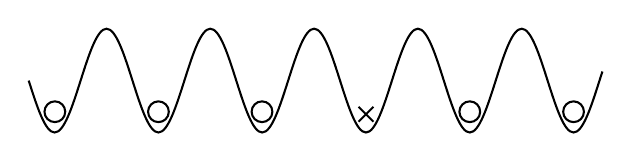
\begin{tikzpicture}[x=0.75pt,y=0.75pt,yscale=-1,xscale=1]
%uncomment if require: \path (0,67); %set diagram left start at 0, and has height of 67

%Shape: Wave [id:dp1825623717070861] 
\draw  [color={rgb, 255:red, 0; green, 0; blue, 0 }  ,draw opacity=1 ] (10,35) .. controls (14.08,47.81) and (17.98,60) .. (22.5,60) .. controls (27.02,60) and (30.92,47.81) .. (35,35) .. controls (39.08,22.19) and (42.98,10) .. (47.5,10) .. controls (52.02,10) and (55.92,22.19) .. (60,35) .. controls (64.08,47.81) and (67.98,60) .. (72.5,60) .. controls (77.02,60) and (80.92,47.81) .. (85,35) .. controls (89.08,22.19) and (92.98,10) .. (97.5,10) .. controls (102.02,10) and (105.92,22.19) .. (110,35) .. controls (114.08,47.81) and (117.98,60) .. (122.5,60) .. controls (127.02,60) and (130.92,47.81) .. (135,35) .. controls (139.08,22.19) and (142.98,10) .. (147.5,10) .. controls (152.02,10) and (155.92,22.19) .. (160,35) .. controls (164.08,47.81) and (167.98,60) .. (172.5,60) .. controls (177.02,60) and (180.92,47.81) .. (185,35) .. controls (189.08,22.19) and (192.98,10) .. (197.5,10) .. controls (202.02,10) and (205.92,22.19) .. (210,35) .. controls (214.08,47.81) and (217.98,60) .. (222.5,60) .. controls (227.02,60) and (230.92,47.81) .. (235,35) .. controls (239.08,22.19) and (242.98,10) .. (247.5,10) .. controls (252.02,10) and (255.92,22.19) .. (260,35) .. controls (264.08,47.81) and (267.98,60) .. (272.5,60) .. controls (277.02,60) and (280.92,47.81) .. (285,35) .. controls (285.47,33.53) and (285.93,32.06) .. (286.4,30.63) ;
%Shape: Circle [id:dp707885383803819] 
\draw  [color={rgb, 255:red, 0; green, 0; blue, 0 }  ,draw opacity=1 ] (17.6,50) .. controls (17.6,47.24) and (19.84,45) .. (22.6,45) .. controls (25.36,45) and (27.6,47.24) .. (27.6,50) .. controls (27.6,52.76) and (25.36,55) .. (22.6,55) .. controls (19.84,55) and (17.6,52.76) .. (17.6,50) -- cycle ;
%Shape: Circle [id:dp7069452766609514] 
\draw  [color={rgb, 255:red, 0; green, 0; blue, 0 }  ,draw opacity=1 ] (67.5,50) .. controls (67.5,47.24) and (69.74,45) .. (72.5,45) .. controls (75.26,45) and (77.5,47.24) .. (77.5,50) .. controls (77.5,52.76) and (75.26,55) .. (72.5,55) .. controls (69.74,55) and (67.5,52.76) .. (67.5,50) -- cycle ;
%Shape: Circle [id:dp008059850674575597] 
\draw  [color={rgb, 255:red, 0; green, 0; blue, 0 }  ,draw opacity=1 ] (117.4,50) .. controls (117.4,47.24) and (119.64,45) .. (122.4,45) .. controls (125.16,45) and (127.4,47.24) .. (127.4,50) .. controls (127.4,52.76) and (125.16,55) .. (122.4,55) .. controls (119.64,55) and (117.4,52.76) .. (117.4,50) -- cycle ;
%Shape: Circle [id:dp5764526829735388] 
\draw  [color={rgb, 255:red, 0; green, 0; blue, 0 }  ,draw opacity=1 ] (217.5,50) .. controls (217.5,47.24) and (219.74,45) .. (222.5,45) .. controls (225.26,45) and (227.5,47.24) .. (227.5,50) .. controls (227.5,52.76) and (225.26,55) .. (222.5,55) .. controls (219.74,55) and (217.5,52.76) .. (217.5,50) -- cycle ;
%Shape: Circle [id:dp8664224311385766] 
\draw  [color={rgb, 255:red, 0; green, 0; blue, 0 }  ,draw opacity=1 ] (267.5,50) .. controls (267.5,47.24) and (269.74,45) .. (272.5,45) .. controls (275.26,45) and (277.5,47.24) .. (277.5,50) .. controls (277.5,52.76) and (275.26,55) .. (272.5,55) .. controls (269.74,55) and (267.5,52.76) .. (267.5,50) -- cycle ;
\draw   (168.9,47.6) -- (176.1,54.81)(176.1,47.6) -- (168.9,54.81) ;




\end{tikzpicture}
 }
    \end{center}
    $$\Rightarrow E_{e_-} = - \mu(N_s-1)$$
\end{enumerate}

\begin{tcolorbox}[breakable, enhanced]
These must be excited states, so we must impose $E_{e_+}, E_{e_-} > E_{g}$:

\begin{equation*}
    \begin{cases}
        E_{e_+} > E_g\\
        E_{e_-} > E_g
    \end{cases}
    \Rightarrow
    \begin{cases}
        U - \mu (\cancel{N_s}+1) > \cancel{-\mu N_s}\\
        - \mu (\cancel{N_s}-1) > \cancel{-\mu N_s}
    \end{cases}
\end{equation*}
\begin{equation*}
    \Rightarrow \begin{cases}
        U > \mu\\
        \mu > 0
    \end{cases}
\end{equation*}

$\Rightarrow$ It must be $U > \mu > 0$ to have consistent excitation and ground states.
\end{tcolorbox}


Now we can compute perturbations. At first order the perturbation is null...
$$\bra{g}\hat{V}\ket{g} = 0 \qquad\qquad \text{because}\;\; \hat{V} \propto \sum_j (\hat{a}^\dag_j + \hat{a}_j)$$
%
... so we go to the second order terms:
\begin{align*}
    \bra{e_+}\hat{V}\ket{g} &= \bra{2_j}-2J\psi(\hat{a}^\dag_j+\cancel{\hat{a}_j})\ket{1_j} = -2J\psi\sqrt2\\
    \bra{e_-}\hat{V}\ket{g} &= \bra{0_j}-2J\psi(\cancel{\hat{a}^\dag_j}+\hat{a}_j)\ket{1_j} = -2J\psi
\end{align*}

\noindent Summing all the contributions up to second order perturbation theory, we end up to
\begin{align*}
    E &= \underbrace{2JN_s\psi^2}_{E_0} + \cancel{E^{(1)}} 
    + \frac{(-2J\psi\sqrt2)^2N_s}{E_g-E_{e_+}}
    + \frac{(-2J\psi)^2N_s}{E_g-E_{e_-}} =\\
    &= 2JN_s\psi^2 + 8\frac{J^2\psi^2}{U-\mu}N_s - 4\frac{J^2\psi^2}{\mu}N_s =\\
    &= 2N_s\psi^2 
    \left( J + \frac{4J^2}{U-\mu} - \frac{2J^2}{\mu} \right)
\end{align*}

Comparing this result with Eq. \ref{eq:landau-bh}, one can find the control parameter $J/U$ that corresponds to the phase transition setting $a_2(J/U) = 0$.


% further reading: https://encyclopedia.pub/entry/33564